\documentclass[UTF8]{ctexart}[a4paper,10pt]
\usepackage[thmmarks]{ntheorem}
\usepackage{amsmath}
\usepackage{amsfonts,amssymb} 
\usepackage{thmtools}
\usepackage[hmargin=2.5cm,vmargin=2.5cm]{geometry}
\usepackage{tikz-cd,tikz}
\usepackage{graphicx,float}
\usepackage{fancyhdr}
\usepackage{fourier-orns}
\usepackage{quiver}
\usepackage{mathrsfs}

%声明环境
\theorembodyfont{\rmfamily}
\newtheorem{example}{例}[section]              
\newtheorem{algorithm}{算法}[subsection]
\newtheorem{theorem}{定理}[section]            
\newtheorem{definition}{定义}[section]
\newtheorem{axiom}{公理}[section]
\newtheorem{property}{性质}[section]
\newtheorem{proposition}{命题}[section]
\newtheorem{lemma}[theorem]{引理}
\newtheorem{corollary}[theorem]{推论}
{
    \theoremheaderfont{\sffamily}
    \newtheorem*{remark}{注解} 
}
\newtheorem{condition}{条件}
\newtheorem{conclusion}{结论}[section]
\newtheorem{assumption}{假设}
{
\theoremstyle{nonumberplain}
\theoremheaderfont{\bfseries}
\theorembodyfont{\normalfont}
\theoremsymbol{\mbox{$\Box$}}
\newtheorem{proof}{证明}
}
%定义命令
\def\N{\mathbb{N}}
\def\Z{\mathbb{Z}}
\def\Q{\mathbb{Q}}
\def\R{\mathbb{R}}
\def\C{\mathbb{C}}
\def\S{\mathbb{S}}
\def\D{\mathbb{D}}
\def\H{\mathbb{H}}
\def\cC{\mathcal{C}}

%页眉设计
\renewcommand 
\headrule{
\hrulefill
\raisebox{-2.1pt}
{\quad{\FourierOrns M T S N}\quad}
\hrulefill}
\pagestyle{fancy}
%极限余极限
\makeatletter
\newcommand{\Colim@}[2]{
  \vtop{\m@th\ialign{##\cr
    \hfil$#1\operator@font lim$\hfil\cr
    \noalign{\nointerlineskip\kern1.5\ex@}#2\cr
    \noalign{\nointerlineskip\kern-\ex@}\cr}}%
}
\newcommand{\Colim}{%
  \mathop{\mathpalette\Colim@{\rightarrowfill@\scriptscriptstyle}}\nmlimits@
}
\makeatother

\makeatletter
\newcommand{\Lim@}[2]{%
  \vtop{\m@th\ialign{##\cr
    \hfil$#1\operator@font lim$\hfil\cr
    \noalign{\nointerlineskip\kern1.5\ex@}#2\cr
    \noalign{\nointerlineskip\kern-\ex@}\cr}}%
}
\newcommand{\Lim}{%
  \mathop{\mathpalette\Lim@{\leftarrowfill@\scriptscriptstyle}}\nmlimits@
}
\makeatother


\makeatletter
\newcommand{\colim@}[2]{%
  \vtop{\m@th\ialign{##\cr
    \hfil$#1\operator@font oli~$\hfil \cr
    \noalign{\nointerlineskip\kern1.5\ex@}#2\cr
    \noalign{\nointerlineskip\kern-\ex@}\cr}}%
}
\newcommand{\colim}{%
  \mathop{\mathrm{c}\mathpalette\colim@{\rightarrowfill@\scriptscriptstyle}\mathrm{\!\!m}}\nmlimits@
}
\makeatother

\makeatletter
\newcommand{\cone@}[1]{%
  \vtop{\m@th\ialign{##\cr
    \hfil$#1\operator@font cone$\hfil\cr
    \noalign{\nointerlineskip\kern1.5\ex@}\cr
    \noalign{\nointerlineskip\kern-\ex@}\cr}}%
}
\newcommand{\cone}{%
  \mathop{\mathpalette\cone@{\scriptscriptstyle}}\nmlimits@
}
\makeatother

%超链接红色
\usepackage[colorlinks,linkcolor=red]{hyperref}

\usepackage{enumerate}


\title{Algebra Topology}
\author{颜成子游}
\begin{document}
\maketitle
\tableofcontents

\quad

笔记来源:J.P.May的《代数拓扑简明教程》。这本书最大的特色是理论性强,叙述简明。因此攥写笔记可以丰富对书的理解,从而提高自己的切实的代数拓扑能力。另外,笔记体系化的可能性并不大,因为时间关系和其他原因。因而只对阅读过的地方做记录,并不保证能读完这本书。(微言大义)
\section{基本群}
基本群读的时候,并没有做笔记,因而这一节暂时只能空缺了。有机会可以补上这一节的笔记。
\section{VK定理}
\subsection{广群(群胚):Groupoid}
为了介绍VK定理,我们首先有必要介绍广群。首先介绍普适一点的定义:
\begin{definition}
    称一个范畴$\cC$是广群,若其每个态射都有逆,意味着其是同构的。所有广群的范畴用$\mathrm{Grpo}$来表示。其态射是两个范畴之间的函子。
\end{definition}
    如果广群的对象只有一个,那么该对象的所有态射显然构成一个群。这也是广群的名字的来源。

    我们聚焦于一类广群:拓扑广群。这类广群由拓扑空间$X$生成,其对象是$X$的每一个点,其态射是两个点之间的道路同伦类。这类广群我们统一记作$\Pi(X)$。因此我们不难想到由如下的函子:
    $$
    \Pi: \mathrm{Top} \to \mathrm{Grpo}
    $$
    这样的函子存在的关键条件在于是否有态射的对应关系。如果$f:X \to Y$是连续映射,那么$\Pi(X)\to \Pi(Y)$是否存在对应的函子呢?

    这样的函子是存在的。设为$F$,则$F(x)=f(x)\in Y$.对于$[x \to x']$的道路同伦类,我们考虑$f[x \to x']$。这是$Y$中的道路同伦类。我们需要验证良定性。若$a$和$b$是$X$中的同伦道路,则$f(a)$和$f(b)$显然是同伦的。这样的对应方式满足的复合性也很容易验证。

    \begin{proposition}
        $\Pi$是一个函子。
    \end{proposition}
    \begin{proposition}
        一个广群是连通的范畴,当且仅当其任意两个对象都是同构的。
    \end{proposition}
    因此$\Pi(X)$是连通范畴当且仅当$X$是道路连通空间。
    \subsection{VK定理的内容}
    我们有两个版本的VK定理,分别对应于群和广群的情况。先叙述广群的情况是更合适的。
    \begin{theorem}[van Kampen]
        设$\mathcal{O}$是$X$的一个道路连通开覆盖,使得其在任意有限交的操作下保持不变。把$\mathcal{O}$看作范畴,对象是里面的开集,态射由集合间的包含关系生成,那么该范畴到$\mathrm{Grpo}$有一个自然的函子。这个函子的余极限是$\Pi(X)$.即:
        $$
        \Pi(X)\cong \Colim_{U \in \mathcal{O}}\Pi(U)
        $$
    \end{theorem}
    \begin{proof}
        由于是余极限,则我们需要先给出$\Pi(U)$到$\Pi(X)$的函子。当然我们肯定先猜测是自然的映入所诱导的函子。

        那么根据余极限的定义,需要对于函子族$\{\eta_{U}:\Pi(U)\to \mathcal{G}\}$给出$\eta:\Pi(X)\to \mathcal{G}$。首先我们知道$U$是开覆盖,所以自然的定义每个点$p \in U$,使得$\eta(p)=\eta_U(p)$即可。当然这里需要验证良定性。事实上若$p \in U\cap V$,则$\eta_U(p)=\eta_{U \cap V}(p)=\eta_{V}(p)$,则良定。

        关键的是定义态射,即对于道路$a:x \to x'$的同伦类$[a]$,注意到$a$作为道路是一个紧集,从而有有限子覆盖$\{U_k\}$。这有限个开集可以把$a$裂成有限条道路的连接,使得这些道路都在某一个$U_k$中。而对于$U_k$中的道路$a_k$,自然可以得到$x_k$到$x_{k+1}$的道路所对应的态射$\eta_{U_k}(a_k) \to \eta_{U_k}(a_{k+1})$。然后所有态射都复合起来,就能得到$a$所对应的值。我们注意到这样做是必须的。

        问题是验证良定性。需要验证这几步操作均不影响:(1)取道路同伦类的代表元。 (2)分裂道路 (3)分别取道路所在同伦类的被映射的态射进行复合。

        首先是同伦类。注意到不同的分裂方式实际上对应了同一个同伦类里面的道路,因此(1)(2)我们只用说明第一个。设$H$是连接同伦,$f$是上端,$g$是下端。则我们可以把$I \times I$分为若干个小正方形,使得每个正方形的像都只在某一个$U_k$中。从而$f$和$g$的每一个小段都是同伦的,这意味着$\eta_{U_k}$作用在上面的像相等。从而我们证明了余极限的成立。
    \end{proof}

    广群的版本虽然简洁,但是我们对于广群范畴并不熟悉,范畴的极限并不是简单的东西。因此我们还是要叙述群的版本。因为群范畴下的极限往往可以写出来的,在实际计算中也有大用。
    \begin{theorem}[van Kampen]
        假设$X$是道路连通空间,给$X$选择一个基点$x$。设$\mathcal{O}$是$X$的开覆盖,并且$x \in U, \forall U \in \mathcal{O}$,满足所有开集都是道路连通并且有限交封闭。同样,将$\mathcal{O}$看作范畴,那么函子:
        $$
        \pi_1(\cdot,x): \mathcal{O}\to \mathrm{Grp}
        $$
        对应的余极限是$\pi_1(X,x)$.即:
        $$
        \Colim_{U \in \mathcal{O}}\pi_1(U,x)=\pi_1(X,x)
        $$
    \end{theorem}
    我们首先不证明这个定理,而介绍一些推论和应用。
    \begin{corollary}
        设$X_i$是一些道路连通的带基点空间,$X$是他们的一点并,$x$是基点。对于$x \in X$和$X_i$,存在$V_i$是包含在$X_i$里面$x$的可缩邻域。则$\pi_1(X)$是所有$\pi_1(X_i)$的余积(自由积)
    \end{corollary}
    \begin{proof}
        设$U_i=X_i \cup \bigcup_{j\neq i}V_j$.$U_i$与任何$X_j$的交集都是开集,因而是开集。此时$U_i$成为$X$的开覆盖,并且以$x$为公共点。构造$X$的开覆盖,这样的开覆盖由$\{U_i\}$和所有的有限交构成。由于任意$U_i$和$U_j$的有限交都是可缩空间,因此这些有限交对于余极限而言毫无帮助。

        另一方面,$U_i$的基本群显然是$X_i$的基本群(这可以用VK定理显而易见的得到),因此$X$的基本群是$\pi_1(X_i,x)$的自由积。
    \end{proof}
    \begin{lemma}
        对于带基点的空间$X,Y$,$\pi_1(X \times Y)=\pi_1(X)\times \pi_1(Y)$。
    \end{lemma}
    \begin{proof}
        这来自于积的泛性质。如果我们能构造交换图成立:
        \begin{figure}[htbp]
            \centering
            \begin{tikzcd}
            &&& {\pi_1(X)} \\
            {\pi_1(X) \times \pi_1(Y)} && {\pi_1(X \times Y)} && {} \\
            &&& {\pi_1(Y)}
            \arrow[from=2-1, to=1-4]
            \arrow[from=2-3, to=1-4]
            \arrow[from=2-3, to=3-4]
            \arrow[from=2-1, to=3-4]
            \arrow["{\exists !}"{description}, dashed, from=2-1, to=2-3]
        \end{tikzcd}
        \end{figure}

    事实上,选取$X \times Y$上的道路同伦类,其代表元投射到$X$和$Y$上自然有$X$和$Y$上的道路,然后得到同伦类。这就是$\pi_1(X \times Y)$到$\pi_1(X)$和$\pi_1(Y)$的投射定义。我们需要说明这是良定义的。这显然,因为$X \times Y$上的同伦限制在$X$上也是同伦。(复合一个$p_X$就万事大吉) 
    
    现在选择$([x],[y]) \in \pi_1(X)\times \pi_1(Y)$,那么什么样的在$X \times Y$上的道路投射到$\pi_1(X)$上才是$[x]$呢。其必然是$x,y$所复合而成的道路。因此这里的唯一存在是自然的。
    \end{proof}
    \begin{definition}
        称$X$是单连通空间,当且仅当其道路连通并且满足$\pi_1(X)=0$.
    \end{definition}
    \begin{proposition}
        设$X =U \cup V$,$U,V,U\cap V$是道路连通空间,并且共用$x \in X$作为同一个基点。若$V$是单连通空间,那么$\pi_1(U)\to \pi(X)$是一个满同态,其核是包含了$\pi_1(U \cap V)$像的最小正规子群。
    \end{proposition}
    \begin{proof}
        设$N$是命题中的正规子群。考虑交换图:
        \begin{figure}[htbp]
            \centering
            \begin{tikzcd}
                & {\pi_1(U)} \\
                {\pi_1(U\cap V)} &&& {\pi_1(X)} & {\pi_1(U)/N} \\
                & {\pi_1(V)=0}
                \arrow["\xi"{description}, dashed, from=2-4, to=2-5]
                \arrow[from=1-2, to=2-4]
                \arrow[from=2-1, to=1-2]
                \arrow[from=2-1, to=3-2]
                \arrow[from=3-2, to=2-4]
                \arrow[from=1-2, to=2-5]
                \arrow[from=3-2, to=2-5]
            \end{tikzcd}
        \end{figure}

        由于$\pi_1(X)$是左半边图的余极限,因此根据泛性质有$\xi:\pi_1(X)\to \pi_1(U)/N$。我们要说明这是一个同构。根据代数学知识,$\pi_1(U)/N$是同态$\pi_1(U \cap V)\to \pi_1(U)$和$\pi_1(U \cap V)\to 0$的推出,因此反过来据泛性质又有$\xi$的逆。从而这是同构。
    \end{proof}
    \subsection{VK定理 群版本的证明}
    \begin{theorem}[van Kampen]

        假设$X$是道路连通空间,给$X$选择一个基点$x$。设$\mathcal{O}$是$X$的开覆盖,并且$x \in U, \forall U \in \mathcal{O}$,满足所有开集都是道路连通并且有限交封闭。同样,将$\mathcal{O}$看作范畴,那么函子:
        $$
        \pi_1(\cdot,x): \mathcal{O}\to \mathrm{Grp}
        $$
        对应的余极限是$\pi_1(X,x)$.即:
        $$
        \Colim_{U \in \mathcal{O}}\pi_1(U,x)=\pi_1(X,x)
        $$
    \end{theorem}
    \begin{proof}
        我们先证明$\mathcal{O}$有限的情况。

        设$G$是任何一个群,且$\eta:\pi_1:\mathcal{O}\to \mathrm{Grp}$是一系列$\mathcal{O}$形状的群的交换图。为了说明泛性质,我们必须说明存在$\tilde{\eta}:\pi_1(X,x)\to G$。并且根据交换图成立,$\tilde{\eta}|_{U}=\eta_{U}$.

        把$\pi_1(X,x)$看作范畴。则$\pi_1(X,x)\to \Pi(X)$存在内射,并且是一个等价。设$J:\Pi(X)\to \pi_1(X,x)$是逆的函子即$F \circ J=\mathrm{id}$.

        因为$\mathcal{O}$是有限的,并且在有限交的运算下保持封闭,因此我们可以做到下面的论断:
        
        若$x,y$都处于$U$中,那么我们可以选择一条从$x$到$y$并且全程在$U$的道路,使得这条道路成为$J$中把$\pi_1(X,y)$映射到$\pi_1(X,x)$的同构。

        从而:
        $$
        \Pi(U)\to \pi_1(U,x) \to G
        $$
        有函子的复合。这样的函子复合满足一个$\mathcal{O}$形的图:$\Pi|\mathcal{O}\to G$.这是因为只要$x,y \in U$,连接他们的道路(以保证同构)就一定在$U$中。

        由于$\Pi(X)$是上面这个图的余极限,因此自然有$\Pi(X) \to  G$的函子。不难想到$\tilde{\eta}:\pi_1(X,x)\to \Pi(X) \to G$是我们想要证明唯一存在的同态(函子)。为了说明我们的想法是正确的,需要计算$\tilde{\eta}|_U$。
        $$
        \tilde{\eta}|_U=( F_U \circ J_U \circ \eta_U)=\eta_U
        $$
        因而泛性质验证完毕。

        接下来考虑一般情况。假设$\mathcal{F}$是这样一个集族:其中的集合是$\mathcal{O}$的有限子集,并且满足有限交封闭。对于$\mathcal{P} \in \mathcal{F}$,设$U_{\mathcal{P}}$是$\mathcal{P}$中开集的并,则$\mathcal{P}$是$U_{\mathcal{P}}$的开覆盖,并且满足有限情况的VK定理。因此:
        $$
        \Colim_{U \in \mathcal{P}}\pi_1(U,x)\cong \pi_1(U_{\mathcal{P}},x)
        $$

        现在把$\mathcal{F}$看作一个范畴,态射由$U_{\mathcal{P}} \subset U_{\mathcal{Q}}$决定。我们断言:
        $$
        \Colim_{\mathcal{P}\in \mathcal{F}} \pi_1(U_{\mathcal{P}},x) \cong \pi_1(X,x)
        $$
        
        这一断言和广群版本的证明很类似。因为每条道路都可以存在有限覆盖,以及$I \times I$的正方形可以拆分为若干个小正方体。

        接下来我们断言:
        $$
        \Colim_{ U \in \mathcal{O}}\pi_1(U,x)\cong \Colim_{\mathcal{P}\in \mathcal{F}}\pi_1(U_{\mathcal{P}},x)
        $$
        
        也就是证明:
        $$
        \Colim_{ U \in \mathcal{O}}\pi_1(U,x)\cong \Colim_{\mathcal{P}\in \mathcal{F}}\Colim_{U\in \mathcal{P}}\pi_1(U,x)
        $$
        对于范畴中的指标范畴换序问题,我们已经了解了。因此我们意图说明下面的极限:
        $$
        \Colim_{(U,\mathcal{P})\in (\mathcal{O},\mathcal{F})} \pi_1(U,x)
        $$
        这个极限和$\Colim_{U \in \mathcal{O}} \pi_1(U,x)$实际上并无二异。按照原书的话来讲,“the system on the right differs
        from the system on the left only in that the homomorphisms $\pi_1(U, x)\to \pi_1(V, x)$
        occur many times in the system on the right, each appearance making the same
        contribution to the colimit.”
    \end{proof}
    这个证明仍有需要注意的地方。为什么不能直接挪用广群的方法证明,而是要这样费尽周折呢?$S_1$是紧集合,那么回路当然也是紧集合。

    答案是我也不知道。这里留一个小小的疑问。
\section{覆叠空间}
\subsection{覆叠空间的定义}
     覆叠空间是代数拓扑中比较重要的一种关系。其提升定理与之后的纤维,上纤维等关系密切,因而学习覆叠空间是必要的。在本章中,我们假设所有的空间都是连通且局部道路连通的,当然这意味着空间本身道路连通。
\begin{definition}[覆叠空间]
    \quad

    设$B$是一个拓扑空间。如果存在拓扑空间$E$和连续满射$p:E \to B$,并且满足:对于$\forall b \in B$,存在$b$的开邻域$V$使得$p^{-1}(U)$是$E$中若干不相交开集$\{U_\alpha\}_{\alpha \in \Lambda}$的并$\bigcup_{\alpha \in \Lambda}U_\alpha$,并且映射$p|_{U_\alpha}:U_\alpha \to U$是同胚,则称$E$是$B$的\textbf{覆叠(复叠,复迭,覆迭)空间},连续映射$p$是对应的覆叠映射。

    我们称满足上述条件的$E$是全空间,$B$是底空间,$F_b=p^{-1}(b)$是覆叠映射$p$的纤维。
\end{definition}
\begin{proposition}
    若$f:A \to B$是连续映射,$D$是$f$和$p$的拉回,即交换图:
    \begin{tikzcd}
        A && D \\
        \\
        B && E
        \arrow["f", from=1-1, to=3-1]
        \arrow["p"', from=3-3, to=3-1]
        \arrow[from=1-3, to=1-1]
        \arrow[from=1-3, to=3-3]
    \end{tikzcd}
    中的$D=\{(a,e)\in A\times E|f(a)=p(e)\}$。此时投射$D \to A$也是覆叠的。
\end{proposition}
\begin{proof}
    首先验证满射。这一点可以由$p$是满射得到:$\forall a \in A,p^{-1}(f(a))$中的任何一个$e$都可以与$a$配对。从这里也可以得到,如果真的是覆叠映射,两个覆叠映射的叶数一样。

    考虑$f(a)$的邻域$V$,则$p^{-1}(V)=\bigcup U_\alpha \subset E$.取其中一个$U_\alpha$,则$p|_{U_\alpha}$是同胚。$U_\alpha$在$D$中的原像是:
    $$
    D_\alpha=\{(a,e)|f(a)=p(e) \in V, e\in U_\alpha\}
    $$
    显然$D_\alpha$投射到$A$上等于$f^{-1}(V)$.连续性是显然的,我们接下来说明限制在$D_\alpha$的投射是同胚,为此只用说明双射。若$(a,e)$和$(a,e')$都在$D_\alpha$中,则$p(e)=p(e')$。由于$p$是同胚,从而$p$是双射,于是$e=e'$。因此单射。满射容易得到。

    因此$D_\alpha$是$f^{-1}(V)$的一个叶子。从而$D \to A$的投射是覆叠映射。
\end{proof}
    这个命题容易让人联想到接下来的上纤维和纤维关于拉回推出的推论。
\subsection{道路提升唯一定理}
\begin{theorem}[提升唯一定理·道路与基本群]
    设$p:E \to B$是覆叠空间。设$b \in B$,$e,e' \in F_b=p^{-1}(b)$。则:
    \begin{enumerate}
        \item 道路$f:I \to B$,$f(0)=b$可以被唯一提升到满足$g(0)=e$的道路$g:I \to E$。其中$e$是给定的$F_b$中的元素。
        \item 同伦的,且起点都在$b$的道路$f \thicksim f'$被提升到同伦的,且起点都在$e$的道路$g \thicksim g'$,因此$g(1)=g'(1)$.
        \item $p_*:\pi_1(E,e) \to \pi(B,b)$是单同态。
        \item $p_*(\pi_1(E,e'))$与$p_*(\pi_1(E,e))$共轭。
        \item 随着$e'$遍历$F_b$,群$p_*(\pi_1(E,e'))$遍历$p_*(\pi_1(E,e))$所有的共轭类。
    \end{enumerate}
  \end{theorem}
  \begin{proof}
    唯一提升定理的证明就不写了,因为重复这样的验证工作没什么意思(指被验证烂了)。
  \end{proof}
  假设$E$的基本群是平凡的,即是单连通空间。此时有一个很有意思的结论:
      
      \begin{proposition}
        设$E$是单连通空间。则$F_b$中的元素与$\pi_1(B,b)$有一个一一对应。
      \end{proposition}
      \begin{proof}
        规定$E$中起点$e$,可以定义映射$\sigma:F_b \to \pi_1(B,b)$,$\sigma(e')$是$E$中$e$到$e'$的道路同伦类。

        这个映射显然是双射。因为$\pi_1(B,b)$的元素只能提升后终点只有一个。并且大家都能提升。
      \end{proof}
      \begin{example}
        $S^n$是$RP^n$的单连通覆叠空间,且$F_b$只有两个元素。因此$\pi_1(RP^2)$只有两个元素,因此$\pi_1(RP^2)=\Z_2$
      \end{example}
      \begin{definition}
        覆叠$p:E \to B$是正则的,若$p_*(\pi_1(E,e))$是正规子群。覆叠是万有的,如果$E$是单连通空间。
      \end{definition}
\subsection{广群的覆叠}
接下来介绍的理论很牛批。因为广群的覆叠本质上就是为了描述覆叠空间中的代数本质。把道路简化为态射,把点简化为对象,这样的想法惊为天人,鬼斧神工般就得到了覆叠空间的代数本质!太厉害辣!
\begin{definition}
设$\cC$是一个范畴,$x$是一个对象。范畴$x\backslash \cC$是这样一个范畴:其对象是从$x$出发的态射$f:x \to y$。其态射$\varphi$是满足$f\circ \varphi:x \to y \to z=g$的$\cC$中的态射。复合和恒等态射都是显然的。若$\cC$是一个广群,此时$\varphi=g\circ f^{-1}$,从而范畴$x\backslash \cC$完全由其对象决定。

设$\cC$是一个小范畴(所有对象可以构成集合)。定义$x$的星集$\mathrm{St}(x)$为$x\backslash \cC$的对象集。记$x$的自态射集合为$\pi(\cC,x)$。
\end{definition}
\begin{definition}[广群的覆叠]
    设$\mathcal{E}$和$\mathcal{B}$是两个小的连通广群。称函子$p:\mathcal{E}\to \mathcal{B}$是一个覆叠,若其在对象集合上是一个满射,并且当限制在$\mathrm{St}(e),\forall e$时得到一个双射:
    $$
    p:\mathrm{St}(e)\to \mathrm{St}(p(e))
    $$
    对于$\mathcal{B}$的对象$b$,记$F_b$是其在$\mathcal{E}$中的原对象集,则$p^{-1}(\mathrm{St}(b))$是以$e$为指标的$\mathrm{St}(e)$集合的不交并。
\end{definition}
\begin{proposition}
    若$p:E \to B$是覆叠空间,那么诱导的函子$\Pi(p):\Pi(E)\to \Pi(B)$是广群的覆叠。
\end{proposition}
\begin{proof}
    对于$e \in E$,$p(e)$是$B$中的元素。$e$往外伸展开的道路同伦类映射到$B$上形成以$b$为起点的道路同伦类。由于道路提升唯一定理和同伦道路提升定理可知,这是一个双射。
\end{proof}
\begin{proposition}
    设$p:\mathcal{E}\to \mathcal{B}$是广群的覆叠,设$b$是$B$的对象,$e$和$e'$是$F_b$中的$\mathcal{E}$的对象。
    \begin{enumerate}
        \item $p:\pi(\mathcal{E},e) \to \pi(\mathcal{B},b)$是单同态。
        \item $p(\pi(\mathcal{E},e'))$与$p(\pi(\mathcal{E},e))$共轭。
        \item 随着$e'$遍历$F_b$,群$p(\pi(\mathcal{E},e'))$遍历$p(\pi(\mathcal{E},e))$所有的共轭类。
    \end{enumerate}
\end{proposition}
\begin{proof}
    这完全是前面定理的对应。不过由于是纯粹的代数问题,我们需要给出证明。

    对于1,由于$p:\mathrm{St}(e) \to \mathrm{St}(b)$是双射,限制在$\pi(\mathcal{E},e)$也应该是双射。从而这里的$p$是单同态。

    对于2,由于$\mathcal{E}$连通,因此选取态射$f:e \to e'$。此时两个群的同构由$f$诱导。$p(f) \in \pi(\mathcal{B},b)$,从而这个诱导的同构由$p$诱导为共轭。

    对于3,$p(\pi(\mathcal{E},e))$的共轭类均由一个$g:b\to b$诱导。根据双射关系,有$g':e \to e'$对应$g$,$e' \in F_b$。从而$g'$被认为是诱导该共轭关系,说明该共轭类是$p(\pi(\mathcal{E},e'))$.
\end{proof}
 
我们注意到$F_b$和$F_b'$之间可能会有很不错的关系。下面的定义和定理深入的研究了这样的关系。
\begin{definition}
    广群覆叠的记号如上。定义纤维变换函子$T=T(p):\mathcal{B} \to \mathrm{Set}$:$T(b)=F_b$。对于$f:b \to b'$,定义映射$T(f):F_b \to F_{b'}$,$T(f)(e)=e'$,其中$g:e \to e'$是$f$的提升。

    $T$成为函子是因为单位态射的提升自然是单位态射,而$T(f\circ g)=T(f)\circ T(g)$也是不难验证的。因为$f \circ g$的提升与$f$,$g$分别提升后复合的末端是一样的。
\end{definition}
纤维变换函子是描述广群覆叠的又一重要工具。比如,其函子性就说明了$T(f)$是$\mathrm{Set}$中的可逆态射,即双射。另外,由于$\mathrm{B}$的对象都是同构的,所以其函子像也都是同构的。换句话说,$F_b$和$F_{b'}$的基数相同。
\subsection{群作用和轨道范畴}
为了研究广群覆叠的关系,下面还要介绍一些东西。

首先我们不再阐述群作用的定义。(最近在每个课程里面都要强调好几次,抽象代数课程再怎么记不住都该熟悉了)称一个群作用是自由的,若$G_s$($s$的迷向子群是平凡的)。也就是$G$对应的同态是单的。

在这里我们主要考虑的是传递作用。这种情况下,$G/G_s$构成的陪集集合与$S$同构。对于$G$的子群$H$,其正规化子$NH$定义为$NH=\{n\in G|n^{-1}Hn=H\}$。容易看出来$H$是$NH$的正规子群,因此我们定义Weyl群:$WH=NH/H$。

下面的引理纯粹是群论性质的(对,意思是我不想证明):
\begin{lemma}
    设$G$传递作用在集合$S$上。记$s \in S$,并且记$H=G_s$.则$WH$同构于群$\mathrm{Aut}_G(S)$。这个记号表示$G$-集合$S$的自同构群。即若$\varphi \in \mathrm{Aut}_G(S)$,则$\varphi(gs)=g\varphi(s),\forall g \in G $.
\end{lemma}
\begin{proof}[我是傲娇]
    对于$[n] \in WH$,定义$\varphi([n])$是这样一个自同构:$\varphi([n])(gs)=gns$.(因为传递作用代表可以记$S=\{gs|g\in G\}$。

    首先验证良定。$gn_1s=gn_2hs=gn_2s$,若$n_1=n_2h,h\in H$。从而良定行显然。

    我们说明这样的对应是同构的。双射:单:若$gn_1s=gn_2s$对于任何$g$都成立,则$n_1s=n_2s$,于是$n_1^{-1}n_2s=s$,即$n_1^{-1}n_2 \in H$,从而$[n_1]=[n_2]$。满射:对于$\varphi(s)=ns$。我们要证明$n \in NH$。注意到$hns=h\varphi(s)=\varphi(hs)=\varphi(s)=ns$,从而$n^{-1}hn\in H$,则$n \in NH$.

    同态:$\varphi([n_1][n_2])(gs)=gn_1n_2s=\varphi([n_2])(gn_1s)=\varphi([n_2])(\varphi([n_1])(gs))$.
\end{proof}

接下来的问题是$G$集合之间的映射
\begin{lemma}
    一个$G-$映射$\alpha:G/H \to G/K$拥有形式$\alpha(gH)=g\gamma K$,其中$\gamma \in G$满足$\gamma^{-1}h \gamma \in K, \forall h \in H$
\end{lemma}
\begin{definition}
    对于群$G$,定义轨道范畴$\mathcal{O}(G)$:对象是$G/H$,态射是$G-$映射。
\end{definition}

因此上面的引理似懂非懂的给出了$\mathcal{O}(G)$的结构。我们用下面的引理来具体化:
\begin{lemma}
    范畴$\mathcal{O}(G)$同构于范畴$\mathcal{G}$,这个范畴的定义是:对象是$G$的子群,态射是不同的子共轭关系:$\gamma^{-1} H \gamma \subset K$,$\gamma \in G$.即$\gamma:H \to K$代表着$\gamma^{-1} H \gamma \subset K$.
\end{lemma}
\begin{proof}
    要定义两个范畴之间的同构函子。对象的定义是自然的。对于$\gamma:G/H \to G/K$,引理说明$\gamma^{-1} H \gamma \subset K$。反之,若$\gamma$满足子共轭关系,那么定义$\alpha(gH)=g\gamma K$,容易验证这是一个$G-$映射。
\end{proof}

我们把群作用的定义拓展到广群。如果广群只有一个对象,则是一个群。此时群作用恰好是$G \to \mathrm{Set}$的一个函子。因此定义小广群的作用为函子$T:\mathcal{B}\to \mathrm{Set}$。对于每个$b$是$\mathcal{B}$的对象,显然$\pi(\mathcal{B},b)$有一个在$T(b)$上的作用。

称$T$是传递的,当且仅当每个$T(b)$上都是传递的。如果$\mathcal{B}$是连通小广群,这个定义可以优化为“存在一个$T(b)$上的作用是传递的。”

\begin{example}
    对于覆叠广群:$p:\mathcal{E}\to \mathcal{B}$,纤维变换函子是从$\mathcal{B}\to \mathrm{Set}$的函子。因此是广群的作用。也就是$\pi(\mathcal{B},b)$作用在$F_b$上。

    对于$e \in F_b$,$e$的迷向子群是:
    $$
    \{g:b \to b|p^{-1}(g):e \to e \in \pi(\mathcal{E},e)\}=p(\pi(\mathcal{E},e))
    $$
    
    这个作用是传递的,因为任何$h:e \to e' \in F_b$都会被$p$映射到$\pi(\mathcal{B},b)$上。

    因此$F_b$实际上是一个$\pi(\mathcal{B},b)$集合,并且$F_b \cong \pi(\mathcal{B},b)/p(\pi(\mathcal{E}),e)$。
\end{example}
\begin{definition}
    广群的覆叠是正则的当且仅当$p(\pi(\mathcal{E},e))$是$\pi(\mathcal{B},b)$的正规子群。是万有的,如果$p(\pi(\mathcal{E},e))=\{e\}$。

    显然覆叠空间的正则和万有与其对应的基本广群覆叠的正则与万有保持一致。

\end{definition}
\begin{proposition}
    广群的覆叠是万有的,当且仅当$\pi(\mathcal{B},b)$自由作用在$F_b$上。此时$F_b$与$\pi(\mathcal{B},b)$同构。这也验证了我们之前所说的,万有覆叠的情况下$\pi_1(B,b)$和$F_b$基数相同。
\end{proposition}
\subsection{广群覆叠的分类定理}
对于一个小的连通广群$\mathcal{B}$,我们想要研究其所有的覆叠广群。因此在之后的几个小节,我们均固定广群$\mathcal{B}$。
\begin{theorem}[覆叠提升基本定理·广群]
    设$p:\mathcal{E}\to \mathcal{B}$是广群的覆叠,并设$\mathcal{X}$是一个广群,$f:\mathcal{X}\to \mathcal{B}$是一个函子。选择一个基对象$x_0\in \mathcal{X}$,设$b_0=f(x_0)$,并设$e_0\in F_{b_0}$。则存在一个函子$g:\mathcal{X}\to \mathcal{E}$使得$g(x_0)=e_0$并且$p\circ g=f$这一事实等价于:
    $$
    f(\pi(\mathcal{X},x_0))\subset p(\pi(\mathcal{E},e_0))
    $$
    当这个条件满足的时候,$g$的存在还是唯一的。
    
    \begin{tikzcd}
        && {\mathcal{E}:e_0} \\
        \\
        {\mathcal{X}:x_0} && {\mathcal{B}:b_0}
        \arrow["p", from=1-3, to=3-3]
        \arrow["f"', from=3-1, to=3-3]
        \arrow["{\exists ! g}", dashed, from=3-1, to=1-3]
    \end{tikzcd}
\end{theorem}
\begin{proof}
    如果$g$存在,则$f(\pi(\mathcal{X}),x_0)=p(g(\pi(\mathcal{X}),x_0))\subset p(\pi(\mathcal{E},e_0))$。因此我们需要说明的是该条件满足时$g$一定唯一存在。

    对于$\mathcal{X}$中的对象$x$,和一个态射$\alpha:x_0 \to x$,设$\tilde{\alpha}$是$\mathrm{St}(e_0)$中唯一的元素满足:$p(\tilde{\alpha})=f(\alpha)$。(提升即可)。如果$g$存在,那么$g(\alpha)$就必须是$\tilde{\alpha}$,因此$g(x)$必须是$\tilde{\alpha}$的终点,即$T(f(\alpha))(e_0)$.

    然而问题是$T(f(\alpha))(e_0)$在$\alpha$变化的过程中会变化吗?换句话说,从$x_0 \to x$的态射很可能不止$\alpha$一个,因此若$\beta:x_0 \to x$,那么$T(f(\beta))(e_0)=T(f(\alpha))(e_0)$能满足吗?

    这一点由条件:$f(\pi(\mathcal{X},x_0))\subset p(\pi(\mathcal{E},e_0))$保证。事实上,此时$\beta^{-1}\circ \alpha$是$\pi(\mathcal{X},x_0)$的元素。从而存在$\gamma \in \pi(\mathcal{E},e_0)$,使得$p(\gamma)=f(\beta^{-1})\circ f(\alpha)$。因此$T(f(\alpha))(e_0)=T(f(\beta))(T(p(\gamma))(e_0))=T(f(\beta))(e_0)$。

    因此我们给出了$g$在对象上的对应。对于态射而言,是显然的。因此$g$不仅存在而且唯一。
\end{proof}
如果是覆叠空间,这个定理反而比较复杂。但我们一旦简化到代数本质上,就显得容易了许多。

接下来我们正式研究覆叠的分类问题。所谓分类,我们可以理解为构建一个范畴关系。对象是所有覆叠广群,而目的是建立态射,最后研究这个范畴的终对象和始对象。那么首先我们定义两个覆叠之间的态射(映射)
\begin{definition}
    称一个函子$g$是广群覆叠的映射,若满足$g:\mathcal{E}\to \mathcal{E}'$并且交换图成立:
    \begin{tikzcd}
        {\mathcal{E}} && {\mathcal{E}'} \\
        \\
        && {\mathcal{B}}
        \arrow["{p'}", from=1-3, to=3-3]
        \arrow["p"', from=1-1, to=3-3]
        \arrow["g", from=1-1, to=1-3]
    \end{tikzcd}
\end{definition}
在这样的定义下,不难验证所有的$\mathcal{E}$构成范畴$\mathrm{Cov}(\mathcal{B})$,我们称之为覆叠范畴。我们用$\mathrm{Cov}(\mathcal{E},\mathcal{E}')$表示两个覆叠空间之间所有的态射。

\begin{lemma}
    $g$作为两个覆叠空间的映射本身也是覆叠。
\end{lemma}
\begin{proof}
    首先说明$g$是满射。取$e' \in \mathcal{E'}$。我们选一个$e\in \mathcal{E}$,则$f:g(e) \to e'$是$\mathcal{E}'$中的态射。把$f$投射到$\mathcal{B}$中,则有$p'(f):p' \circ g(e) \to p'(e')$。这个态射可以被提升到$\mathcal{E}$上,并且以$e$为起点。这个态射的终点被$g$作用后必然是$e'$。
    
    其次,$e$,$e'$,$b$三个点的星集是具有双射的集合。
\end{proof}
      覆叠基本定理给出了两个覆叠之间存在态射的充要条件。叙述如下:
      
\begin{theorem}
        设$p:\mathcal{E}\to \mathcal{B}$和$p':\mathcal{E}' \to \mathcal{B}$都是广群覆叠。选择$b \in \mathcal{B},e \in \mathcal{E},e'\in \mathcal{E'}$使得$p(e)=b=p'(e')$。那么存在一个映射$g:\mathcal{E}\to \mathcal{E'}$并且满足$g(e)=e'$当且仅当:
        $$
        p(\pi(\mathcal{E},e)) \subset p'(\pi(\mathcal{E'},e')) 
        $$  
        并且此时$g$的存在是唯一的。也就是说,如果$g,g'$同时满足$g(e)=g'(e)$,则$g=g'$。
        
        $g$是同构当且仅当上述的包含是相等。因此$\mathcal{E}$和$\mathcal{E}'$是同构的当且仅当$p(e)=p'(e')$的时候有$p(\pi(\mathcal{E},e))$和$p'(\pi(\mathcal{E}',e'))$是共轭的。
\end{theorem}

因此万有覆叠是任何覆叠的覆叠,并且在同构意义下唯一。我们接下来要做的是证明其存在。

放在一边。下面的定理仍然是值得注意的:
\begin{theorem}
    覆叠广群的记法如上。选择基点$b\in \mathcal{B}$,并记$G=\pi(\mathcal{B},b)$。则下面的两个集合存在双射:
    \begin{enumerate}
        \item $F_b$到$F_b'$的所有$G$映射。
        \item $\mathrm{Cov}(\mathcal{E},\mathcal{E'})$。
    \end{enumerate}
    并且这个双射是由$g$诱导的。即$g$限制在$F_b$上成为$G$映射。
\end{theorem}
\begin{proof}
    需要说明两点:1.任何$g$限制在$F_b$都成为到$F_{b'}$的$G$映射。2.任何$G$映射都能被延拓为某个$g$。

    先说明第一点。设$g$是一个广群覆叠之间的映射。取$e'=g(e),e\in F_b,e' \in F_{b'}$.则$F_b$与$F_{b'}$被表示为:$G/p(\pi(\mathcal{E},e))$和$G/p'(\pi(\mathcal{E}',e'))$。我们知道$G$映射的形式是$\alpha(gH)=g\gamma K$,$\gamma^{-1} H \gamma \subset K$.

    对于$he$,$g$作用在上面得到的结果是$hg(e)=he'$。因为$e \to he$,$h:b \to b$,$e' \to he'$是三个对应的态射。从而其末尾也相互对应。这说明$g$限制在上面是$G$映射。

    现在考虑双射问题。如果$g$与$g'$不同,那么在每个$e$上$g$与$g'$的值都不同。从而诱导出的$g(he)$不是$F_b'$中的同一个元素。这意味着限制在$F_b$上$g$与$g'$不同。对于任何$F_b$与$F_b'$的$G$映射$\alpha$,意味着$\alpha(ge)=ge'$。从而$\alpha(e)= e' \in F_b'$。

    根据前面的定理,我们要验证$p(\pi(\mathcal{E},e))$在$p(\mathcal{E}',e')$中。这是$e$和$e'$的迷向子群。由于$\alpha(e)=e'$,因此$e$的迷向子群显然是$e'$迷向子群的子集。故根据定理知存在延拓后的$\alpha$。
\end{proof}

这个定理说明$F_b$和$F_b'$中的$G$映射就唯一决定了所有的$g$覆叠。由纤维决定了映射,这是覆叠广群巧妙的性质。

我们用$\mathrm{Aut}(\mathcal{E})$表示$\mathcal{E}$自身的覆叠映射全体。这显然构成一个群。这不一定是同胚,因为$H$和$H'$作为共轭子群,可能存在$H <H'$。

下面的推论在上述定理的支持比较显然。只用验证其运算保持不变即可。
\begin{corollary}
    设$p$是覆叠,选择一个$b$作为$\mathcal{B}$的对象。简记$G=\pi(\mathcal{B},b)$和$H=p(\pi(\mathcal{E},e))$.那么$\mathrm{Aut}(\mathcal{E})$同构于$F_b$作为$G$集合的自同态群,即$WH$.

    如果$p$是正则覆叠,即$H$是正规子群,此时其正规化子为$G$,因此$WH=G/H$。如果$p$是万有覆叠,则$H$平凡,正规化子也为$G$,$WH=G$。
\end{corollary}
\subsection{广群覆叠的构造}
我们研究清楚了广群覆叠之间的关系。但对于具体的范畴,只研究态射而不研究对象,就好像是母单天天打galgame而不去恋爱实践一样,只是空中楼阁。因此我们要解决的问题是,到底有哪些广群覆叠?

首先根据之前的研究,我们知道最多只有一个同构类的覆叠广群对应$\pi(\mathcal{B},b)$的共轭子群类。但实际上至多这个词可以被删去。我们将证明所有的男生都可以如愿找到女(男)朋友(指所有的共轭类都能对应一个广群的覆叠)。

\begin{theorem}
    对于广群$\mathcal{B}$,选择基对象$b$,记$G=\pi(\mathcal{B},b)$。则存在一个函子$\mathcal{E}()$:
    $$
    \mathcal{E}():\mathcal{O}(G)\to \mathrm{Cov}(B)
    $$
    使得上述两个范畴是等价范畴。对于$G$的子群$H$,覆叠$p:\mathcal{E}(G/H) \to \mathcal{B}$有一个典范的基对象$e$,使其处于$b$的纤维中,并且:
    $$
    p(\pi(\mathcal{E}(G/H),e))=H
    $$

    此时,$F_b=G/H$,并且对于映射$\alpha:G/H \to G/K$,把$\mathcal{\alpha}$限制在$F_b$正好是$\alpha$本身。
\end{theorem}
\begin{proof}
    我们只说明基本思路。具体的验证工作省略。注意到$\mathrm{St}_{\mathcal{E}(G/H)}(e)$与$\mathrm{St}_\mathcal{B}(b)$作为集合来说有同构,因此不管$H$如何,$\mathrm{St}(e)$在双射的意义下是一样的。但是这些态射的终点可以根据$H$的情况发生变化。即我们可以重复掉一些态射来“节省”空间。例如若$H$是平凡群,此时$\mathcal{E}(G)$是万有覆叠,从而$e$和$e'$只有一个态射。因此每个终点和每个态射一一对应。若$H$是$G$本身,此时$\mathcal{E}(G/G)$是$\mathcal{B}$本身。因此$e=b$,从而$b$到$b'$的态射集合是$\pi(\mathcal{B},b)$的复制。终点和态射的关系也是明朗的。

    对于一般的$H$,定义$G$作用在$\mathrm{St}(b)$上。方式为先转一圈再发射出去。则等价关系$x \thicksim y:hx=y,h \in H$存在。商去这个关系:$\mathrm{St}(b)/H$,我们将该集合作为$\mathcal{E}(G/H)$的对象集合。

    接下来定义这个范畴的态射。取某个对象的代表元$f:b \to b'$和$g: b \to b''$。两个对象之间的态射定义为$ g \circ h \circ f^{-1}$,$h \in H$。从而态射集合与$H$有一一对应。容易验证上述定义满足范畴的要求。并且形成广群。

    我们需要典范的基对象。设$e$是$\mathrm{id}_b$所在的等价类,则$\pi(\mathcal{E}(G/H),e)$是$\mathrm{id}_b$到自身的态射集合,即$H$本身。

    设覆叠$p$是把$fH$映射到其末尾,把态射映射为$\mathcal{B}$中一样的态射。则$p(H)=H$。只需要验证$p$是覆叠。为此,从$fH$出发的态射与$b'$出发的态射需要存在一一对应。前者到后者通过$p$对应,而取$g:b' \to b''$是后者的某一个态射,则$g \circ f$是从$b$到$b''$的态射。其所在的等价类与$fH$的等价类之间显然有态射$g$。因此这是双射。

    最后说明$G/H$和$G/K$的映射$\alpha$.定义$\mathcal{E}(\alpha)$把$fH$映射到$fgK$。其中$\alpha(aH)=agK,\forall aH \in G/H$.把态射$f' \circ h \circ f^{-1}$映射到同样的态射$f'g \circ g^{-1}hg \circ g^{-1}f^{-1}$。因为$g^{-1}hg \in K$。接下来的验证:函子性,限制$F_b$上等问题就省略了。
\end{proof}
\subsection{覆叠空间的分类定理}
覆叠空间的分类定理,即考虑同一个空间$B$的所有覆叠空间$\mathrm{Cov}(B)$之间的关系。注意到我们在研究关系,因此可以来猜测这样的关系本质是代数的,即之前广群的定理全部可以照搬过来。也就是说,我们完全可以把推gal的经验用在和现实的女孩子谈恋爱上。(如果已经有女朋友了)

可惜的是,空间的构造并非代数的,也就是之后的一节:覆叠空间的构造本身是拓扑的构造,即代数并不能有一个很好的相似方法来做覆叠空间。也就是说,就算你gal打的再多,要是连女朋友都找不到,也白搭。
\begin{theorem}[覆叠提升基本定理·拓扑空间]
    设$p:E\to B$是拓扑空间的覆叠,并设$X$是一个拓扑空间,$f:X\to B$是连续映射。选择一个基点$x_0\in X$,设$b_0=f(x_0)$,并设$e_0\in F_{b_0}$。则存在一个连续映射$g:X\to E$使得$g(x_0)=e_0$并且$p\circ g=f$这一事实等价于:
    $$
    f_*(\pi_1(X,x_0))\subset p_*(\pi_1(E,e_0))
    $$
    当这个条件满足的时候,$g$的存在还是唯一的。
    
    \begin{tikzcd}
        && {E:e_0} \\
        \\
        {X:x_0} && {B:b_0}
        \arrow["p", from=1-3, to=3-3]
        \arrow["f"', from=3-1, to=3-3]
        \arrow["{\exists ! g}", dashed, from=3-1, to=1-3]
    \end{tikzcd}
\end{theorem}
\begin{proof}
    若$g$存在,显然有包含关系。

    若包含关系满足,则广群覆叠$\Pi(p):\Pi(E)\to \Pi(B)$也有类似的包含关系,因此存在函子$g$。$g$可以看作映射,但是需要验证$g$的连续性。若$y \in X$,$g(y) \in U$,$U$是$E$的开集。则存在更小的$g(y)$的开邻域$U'$使得$p$同胚的把$U'$映射到$B$上开集$V$。若$W$是任何$y$的道路连通邻域使得$f(W)\subset V$,则$g(W)\subset U'$。这说明$g$是连续的。
\end{proof}
\begin{definition}
    称一个连续函数$g$是拓扑空间覆叠之间的映射,若满足$g:E\to E'$并且交换图成立:
    \begin{tikzcd}
        {E} && {E'} \\
        \\
        && {B}
        \arrow["{p'}", from=1-3, to=3-3]
        \arrow["p"', from=1-1, to=3-3]
        \arrow["g", from=1-1, to=1-3]
    \end{tikzcd}
\end{definition}
同样有类似的记号$\mathrm{Cov}(B)$,$\mathrm{Cov}(E,E')$.

\begin{lemma}
    覆叠空间$E \to E'$的映射自身也是覆叠。
\end{lemma}
\begin{proof}
    $e'$和$g(e)$都是$E'$的点,因此有道路连接。该道路投射到$B$上,再提升到$E$上并要求起点是$e$。则终点的$g$像是$e'$.从而$g$满射。$p'(e')$是$B$的点,从而有一个$U$满足$p^{-1}(U)$和$p'^{-1}(U)$是基本的。$e'$属于$p'^{-1}(U)$中的某个部分$V$,则$V$是基本的。这一点可以由道路连通的角度来看。
\end{proof}

覆叠基本定理给出了两个覆叠之间存在态射的充要条件。叙述如下:
      
\begin{theorem}
        设$p:E\to B$和$p':E' \to B$都是覆叠。选择$b \in B,e \in E,e'\in E'$使得$p(e)=b=p'(e')$。那么存在一个映射$g:E\to E'$并且满足$g(e)=e'$当且仅当:
        $$
        p_*(\pi_1(E,e)) \subset p'_*(\pi_1(E',e')) 
        $$  
        并且此时$g$的存在是唯一的。也就是说,如果$g,g'$同时满足$g(e)=g'(e)$,则$g=g'$。
        
        $g$是同胚当且仅当上述的包含是相等。因此$E$和$E'$是同胚的当且仅当$p(e)=p'(e')$的时候有$p_*(\pi_1(E,e))$和$p'_*(\pi_1(E',e'))$是共轭的。
\end{theorem}
\begin{corollary}
    万有覆叠在存在的情况下是同胚唯一的。
\end{corollary}

基本群能够决定覆叠空间之间的关系,这是代数拓扑中少有的事情。这很不典型。但是下面的定理或许能让我们初见其端倪:
\begin{theorem}
    基本广群函子诱导双射:
    $$
    \mathrm{Cov}(E,E') \to \mathrm{Cov}(\Pi(E),\Pi(E'))
    $$
\end{theorem}
\begin{proof}
    由上述定理显然。
\end{proof}

把覆叠间的映射限制在$F_b$上自然得到$F_b$到$F_b'$的映射。这是$G$映射。而$F_b$到$F_b'$的$G$映射都自然能诱导覆叠间的映射。这是局部与整体的巧妙联系。
\begin{theorem}
    覆叠空间记法如上。选择基点$b\in B$,并记$G=\pi_1(B,b)$。则下面的两个集合存在双射:
    \begin{enumerate}
        \item $F_b$到$F_b'$的所有$G$映射。
        \item $\mathrm{Cov}(E,E')$。
    \end{enumerate}
    并且这个双射是由映射$g$诱导的。即$g$限制在$F_b$上成为$G$映射。
\end{theorem}
\begin{proof}
    $G$作用在$F_b$上,意味着一种提升。即$e$到$f e$的道路同伦类被$p_*$映射为$f$。考虑$g(fe)$与$f g(e)$。$g(e)$到$f g(e)$的道路同伦类,$e$到$fe$的道路同伦类,被映射为$B$上的$f$。自然有$g(fe)=fg(e)$。这说明$g$限制后是$G$映射。

    不同的$g$限制在$F_b$上结果必然不同。因为若$g(e)=g'(e)=e'$,则,满足该条件的$g$只能有一个。

    对于$F_b$到$F_b'$的$G$映射$\alpha$,我们需要验证包含关系。这是$F_b$和$F_b'$的迷向子群。由于$\alpha$是$G$映射,因此迷向子群显然包含关系。
\end{proof}
类似的,我们用$\mathrm{Aut}(E)$表示$E$自身的覆叠映射全体。这显然构成一个群。这不一定是同胚,因为$H$和$H'$作为共轭子群,可能存在$H <H'$。
\begin{corollary}
    设$p$是覆叠,选择一个$b$作为$B$的对象。简记$G=\pi_1(B,b)$和$H=p(\pi_1(E,e))$.那么$\mathrm{Aut}(E)$同构于$F_b$作为$G$集合的自同态群,即$WH$.

    如果$p$是正则覆叠,即$H$是正规子群,此时其正规化子为$G$,因此$WH=G/H$。如果$p$是万有覆叠,则$H$平凡,正规化子也为$G$,$WH=G$。
\end{corollary}

\subsection{覆叠空间的构造}
这一节我们将介绍几个定理。证明是省略的,因为其本身并没有太多的帮助。只需要记住这些定理的结果,覆叠空间的基本性质就被拿捏了。
\begin{definition}
    称空间$B$是局部半单连通的,若任意$b \in B$都有一个邻域$U$使得$\pi_1(U,b) \to \pi_1(B,b)$是平凡同态。
\end{definition}
该定义显然是万有覆叠存在的必要条件。因为其基本邻域与$E$中某开集同胚,而该开集到$B$的映射将所有道路同伦类变为$1$.

但实际上这个条件保证了万有覆叠的存在:
\begin{theorem}
    若$B$连通,局部道路连通,局部半单连通,则$B$有万有覆叠。
\end{theorem}
\begin{proof}
    只说一句,考虑广群,我们起码会知道这个万有覆叠空间的点都是$b$到其他点的道路同伦类。问题的难点在于拓扑的构造。因为代数只能得到广群,广群不给拓扑是形成不了空间的。
\end{proof}

\begin{lemma}
    设$X$是$G$空间,则轨道范畴到$\mathrm{Top}$有函子$X/(-)$。
\end{lemma}
\begin{proof}
    $G/H$将被映射为$X/H$.若$G/H \to G/K$有$G$映射$\alpha$,则$X/H \to X/K$有连续函数$\alpha$:$\alpha(Hx)=K\gamma^{-1}x$.其中$\alpha(H)=\gamma K$。
\end{proof}
\begin{proposition}
    设$p:E \to B$是覆叠,$\mathrm{Aut}(E)$传递的作用在$F_b$上。则覆叠是正则的,并且$E/\mathrm{Aut}(E)$同胚于$B$。
\end{proposition}
\begin{proof}
    
\end{proof}
\begin{theorem}
    对于$B$,选择基点$b$,记$G=\pi_1(B,b)$。则存在一个函子$E(-)$:
    $$
    E(-):\mathcal{O}(G)\to \mathrm{Cov}(B)
    $$
    使得上述两个范畴是等价范畴。对于$G$的子群$H$,覆叠$p:E(G/H) \to B$有一个典范的基点$e$,使其处于$b$的纤维中,并且:
    $$
    p_*(\pi_1(E(G/H),e))=H
    $$

    此时,$F_b=G/H$,并且对于映射$\alpha:G/H \to G/K$,把$E(\alpha)$限制在$F_b$正好是$\alpha$本身。
\end{theorem}
因此$\pi_1(B,b)$实际上承担了许多责任。下面有典范的范畴等价:
\begin{tikzcd}
	& {\mathcal{O}(\pi_1(B,b))} \\
	{\mathrm{Cov}(B)} && {\mathrm{Cov}(\Pi(B))}
	\arrow["{E(-)}"', from=1-2, to=2-1]
	\arrow["{\mathcal{E}(-)}", from=1-2, to=2-3]
	\arrow["\Pi", from=2-1, to=2-3]
\end{tikzcd}

\section{图}
图是一个神秘的存在。其是基本群和覆叠空间的应用。我们笔记从简,只记录基本定理和证明思路,因为其本身不是主线。
\section{紧致生成空间——CGWH空间}
拓扑空间繁多复杂。许多奇怪的拓扑并不违背点拓的规则,但是于具体问题无济于事。代数拓扑对空间进行了若干要求,以保证研究问题的流畅性以及理论的协调性。

下面的内容真的好点拓啊,看的我头皮发麻呜呜呜。大概就一天补一个命题的证明,花一周时间把这章写完吧。

\textbf{注意:若无特殊说明,之后约定所谓“紧空间”是指紧且Hausdorff的空间}。

\subsection{紧致生成空间的定义}
\begin{definition}
    $X$被称作弱Hausdorff的,若对于任何紧空间$K$和连续映射$g:K \to X$,$g(K)$是$X$的闭子集。
\end{definition}
\begin{lemma}
    当$X$是弱Hausdorff空间的时候,$g(K)$也是紧空间。
\end{lemma}
\begin{proof}
    紧性显然。问题是验证Hausdorff性质。如果$g$是闭映射,那么容易知道$T_4$空间是闭连续保持的,因而$g(K)$是Hausdorff空间。$g$是闭映射,因为$F \subset K$是闭集,则$F$也是紧Hausdorff空间,因此$g(F)$是$X$中闭集。而$g(K)$也是闭集,则$g(F)$是$g(K)$中闭集。
\end{proof}

弱Hausdorff性质是介于$T_1$和Hausdorff之间的分离性质。显然Hausdorff能推得弱Hausdorff,而$T_1$要求单点是闭集。由于单点必然是紧Hausdorff的,因此其必然是闭集。

\begin{definition}
    $X$的子空间$A$被称作是紧致闭的,若对于任意紧空间$K$和$g:K \to A$,$g^{-1}(A)$是$K$中的闭集。若$X$本身是弱Hausdorff的,那么该条件等价于$A$与$X$的任意紧子集相交都是闭集。
\end{definition}
\begin{proof}
    
\end{proof}
\begin{definition}
    $X$是k空间,若每个紧致闭的子集都是闭集。注意这里的紧致闭集不是闭+紧,是上面的定义。我们约定使用紧致且闭来表达闭+紧的含义。
\end{definition}

\begin{definition}
    $X$是紧致生成的空间,若其是一个弱Hausdorff的k空间。
\end{definition}
\begin{example}
    任何一个局部紧,第一可数的空间是紧致生成的空间。任何弱Hausdorff且第一可数的空间是紧致生成的空间。
\end{example}
\begin{proof}
    
\end{proof}
\begin{lemma}
    若$X$是紧致生成的空间,$Y$是任意空间,那么函数$f:X \to Y$是连续的当且仅当对于$X$的任何紧子集$K$,$f|_K$是连续的。
\end{lemma}
\begin{proof}
    
\end{proof}
引理有力的说明了紧致生成空间名字的由来:这个空间的拓扑和紧集有一种相容。所有的性质只由紧集决定。很多时候我们遇到的空间不是$k$空间,但是经过以下处理可以得到$k$空间。
\begin{proposition}
    设$X$是一个空间。给$X$赋予一个新的拓扑:$A$是$X$中的闭集,当且仅当其在原拓扑中是紧致闭的。这个拓扑的定义是良定的。
\end{proposition}
\begin{proof}
    
\end{proof}
我们把上述操作称为$k$化,得到的空间记为$kX$。从而有自然恒等映射$kX \to X$。这个映射显然是连续的。
\begin{proposition}
    若$X$是弱Hausdorff空间,则$kX$也是弱Hausdorff空间。从而弱Hausdorff空间的$k$化空间是紧致生成空间。
\end{proposition}
\begin{proof}
    回忆弱Hausdorff空间的定义。设$g:K \to kX$是连续函数且$K$是紧空间。我们想要证明$g(K)$是闭集。注意到$g(K)$作为$X$的子集来说是闭集($\mathrm{id}\circ g$同样是连续函数,且$\mathrm{id}\circ g(K)=g(K)$),则$g(K)$显然是$kX$中的闭集。
\end{proof}
\begin{proposition}
    $X$和$kX$拥有完全相同的紧子集。
\end{proposition}
\begin{proof}
    
\end{proof}

现在我们考虑弱Hausdorff和Hausdorff的相似之处。用$X \times_c Y$表示$X$和$Y$的一般乘积空间,用$X \times Y$表示$X \times _c Y$的$k$化。
\begin{proposition}
    若$X$和$Y$都是弱Hausdorff空间,则$X \times Y=kX \times kY$.若$X$是局部紧空间且$Y$是紧致生成空间,则$X \times Y=X \times_c Y$
\end{proposition}
\begin{proof}
    
\end{proof}
\begin{lemma}
    设$X$是$k$空间,那么$X$是弱Hausdorff空间当且仅当$\Delta X=\{(x,x)\} \subset X \times X$是闭集。
\end{lemma}
\begin{proof}
    
\end{proof}
\subsection{紧致生成空间范畴}
我们先说明本章的大标题——CGWH(compactly generated weak Hausdorff)。由于不同书对紧致生成空间,紧的定义有区别。如果不认为紧致=紧+Hausdorff,那么我们也没有理由认为紧致生成蕴含着弱Hausdorff。紧致生成空间有另外的定义:
\begin{definition}[不作为本笔记的一般定义]
    称一个空间是紧致生成空间,若$A\subset X$是闭集当且仅当对于$X$的任何紧子集$X$,$A\cap K$都是闭集。称一个空间是豪斯多夫紧致生成空间(k空间),若$A\subset X$是闭集当且仅当对于$X$的任何紧豪斯多夫子集$X$,$A\cap K$都是闭集。称一个空间是紧致生成豪斯多夫空间,若其是紧致生成的,并且豪斯多夫。
\end{definition}
因而在这种前提下,CGWH空间,即紧致生成弱Hausdorff空间应该有定义:豪斯多夫紧致生成且弱Hausdorff的空间。这一个定义与之前的定义是一致的,即在弱Hausdorff的条件下:
\begin{proposition}
    若$X$是弱Hausdorff空间,则$X$是$k$空间当且仅当其的每个紧致闭集合都是闭集。
\end{proposition}

暂且不表。以后我们记录紧致生成的时候均代表CGWH空间。

一般的拓扑范畴$\mathrm{Top}$有一些不好的性质。比如商空间中。但考虑紧致生成空间可以避免:
\begin{proposition}
    设$X$是紧致生成空间,$\pi:X \to Y$是商映射,那么$Y$是紧致生成的当且仅当$(\pi \times \pi)^{-1}(\Delta Y)$是$X \times X$中的闭集。
\end{proposition}
可以对该命题做如下通俗的解释:一个紧致生成空间的商空间,若通过一个“闭的等价关系”诱导,则是紧致生成的空间。

\begin{proposition}
    若$X$和$Y$是紧致生成空间,$A$是$X$的闭子集,并且$f: A \to Y$是任意连续映射,则推出空间$Y \cup_{f} X$是紧致生成的空间。
\end{proposition}

\begin{proposition}
    若$\{X_i\}$是一系列紧致生成空间,并且包含映射$X_i\to X_{i+1}$均为闭的像集,则余极限$\Colim X_i$是紧致生成的。
\end{proposition}

接下来我们给出若干范畴的定义。这样是为了更好的说明CGWH空间的优点。
\begin{definition}
    重新定义$\mathrm{Top}$为所有紧致生成空间的范畴,$\mathrm{Top*}$为对应的带基点的范畴。记$w\mathrm{Top}$是所有弱Hausdorff空间的范畴,从而我们有函子:$k:w \mathrm{Top} \to \mathrm{Top}$和遗忘函子$j:\mathrm{Top}\to w\mathrm{Top}$.
\end{definition}
\begin{proposition}
    $(j,k)$是伴随函子。即$k$是$j$的右伴随,$j$是$k$的左伴随。
\end{proposition}
\begin{proof}
    
\end{proof}
注意到$w\mathrm{Top}$中,极限存在。即按照最一般的拓扑空间来看,弱Hausdorff空间的极限仍然是弱Hausdorff的。但是k空间不具有这样的性质。由于$k$是右伴随,因此保极限。从而我们可以先作遗忘函子,然后得到极限,再作用$k$。这样就可以得到$\mathrm{Top}$中的极限。这样的极限做法在集合上没有变化,唯一要注意的是拓扑发生的变化。

\begin{definition}
    对于两个紧致生成空间$X$,$Y$,记$Y^X$表示从$X$到$Y$的所有连续函数组成的集合。其拓扑由标准的紧开拓扑k化得到。所谓紧开拓扑,是指由下列集合作为子基组成生成的拓扑:
    $$
    \{U\subset Y,K \subset X|\{f|f(K)\subset U\}\}
    $$
    其中$U$是$Y$的开集,$K$是$X$的紧子集。
\end{definition}
\begin{proposition}[乘积空间的伴随]
    对于紧致生成空间$X,Y,Z$,典范的双射:
    $$
    Z^{X \times Y}\cong (Z^Y)^X
    $$
    是一个同胚。
\end{proposition}

从下节开始,所有的空间都被认为是紧致生成空间(CGWH),由此我们不再论述其前提。关于CGWH空间范畴,可以见Wiki。有详细的性质论述。
\section{上纤维}
纤维与上纤维是对偶的两组概念,其中的证明很多都是可以通过改变箭头方向,及乘积为指数等办法而复制证明。我们只证明对偶中的一个,另一个在纸上会做验证。

\subsection{上纤维的定义}
\begin{definition}
    称一个连续函数$i:A \to X$是上纤维,若其满足同伦拓展性质(homotopy extension property:HEP).这意味着若下列交换图中,若已经有:$h \circ i_0=f \circ i$,则存在$\tilde{h}$使得该图交换。
\begin{figure}[htbp]
    \centering
    \begin{tikzcd}
        A && {A\times I} \\
        \\
        X && {X \times I} \\
        &&& Y
        \arrow["i", from=1-1, to=3-1]
        \arrow["{i_0}", from=3-1, to=3-3]
        \arrow["{i_0}", from=1-1, to=1-3]
        \arrow["{i\times \mathrm{id}_I}"', from=1-3, to=3-3]
        \arrow["f", from=3-1, to=4-4]
        \arrow["h", from=1-3, to=4-4]
        \arrow["{\exists \tilde{h}}"{description}, dashed, from=3-3, to=4-4]
    \end{tikzcd}
\end{figure}
\end{definition}
简单地说,如果$A$到$Y$有同伦,并且起点函数可以延拓为整个$X$的函数,那么整个同伦都可以被提升。

我们并不要求$\tilde{h}$具有唯一性。事实上其很多时候都不唯一。这个图也可以改写为紧凑的形式:\begin{tikzcd}
	A && {Y^I} \\
	\\
	X && Y
	\arrow["i", from=1-1, to=3-1]
	\arrow["f", from=3-1, to=3-3]
	\arrow["{p_0}"', from=1-3, to=3-3]
	\arrow["{\tilde{h}}"{description}, dashed, from=3-1, to=1-3]
	\arrow["h"', from=1-1, to=1-3]
\end{tikzcd} 原因是$A \times I \to Y$与$A \to Y^I$是同胚的。$p_0(\xi)=\xi(0)$.

\begin{lemma}
    上纤维映射的推出也是上纤维。即对于$i: A \to X$是上纤维,$g:A \to B$是连续函数,那么诱导映射$B \to B\cup_g X$也是上纤维。
\end{lemma}
\begin{proof}
    交换图表道尽一切:
    \begin{figure}[htbp]
        \centering
        \begin{tikzcd}
            & {} \\
            A &&&& {A \times I} \\
            & B && {B\times I} \\
            && Y \\
            & {B \cup_g X} && {(B\cup_g X)\times I} \\
            X &&&& {X \times I}
            \arrow[from=3-2, to=5-2]
            \arrow[from=3-4, to=5-4]
            \arrow[from=3-2, to=3-4]
            \arrow[from=5-2, to=5-4]
            \arrow[from=5-2, to=4-3]
            \arrow[from=3-4, to=4-3]
            \arrow[from=2-1, to=3-2]
            \arrow[from=2-1, to=6-1]
            \arrow[from=6-1, to=5-2]
            \arrow[from=6-1, to=6-5]
            \arrow[from=2-1, to=2-5]
            \arrow[from=2-5, to=6-5]
            \arrow[from=6-5, to=5-4]
            \arrow[from=2-5, to=3-4]
            \arrow[curve={height=-18pt}, dashed, from=6-5, to=4-3]
            \arrow[dashed, from=5-4, to=4-3]
        \end{tikzcd}
    \end{figure}

    事实上,弯曲的虚线是$A \to X$的上纤维定义。直的虚线来自于$(B\cup_g X) \times I=(B\times I)\cup_{g\times \mathrm{id}_I} (X \times I)$,从而右边的题型是推出,因此根据推出的性质有该直虚线。
\end{proof}
\subsection{映射柱}
映射柱和映射锥是相当重要的概念。其来自于上纤维。对于映射$i:A\
to X$,定义其映射柱$Mi$是$i$和$A \to A \times I$的推出:
$$
Mi\equiv X\cup_i(A \times I)
$$
一般我们把$a \mapsto (a,0)$,意味着粘的地方是$A \times I$的底层(0层)。

如果交换图成立,我们立马就可以意识到上纤维的成立:
\begin{tikzcd}
	A && {A\times I} \\
	& Mi \\
	X && {X \times I}
	\arrow[from=1-1, to=3-1]
	\arrow[from=3-1, to=2-2]
	\arrow[from=1-1, to=1-3]
	\arrow[from=1-3, to=2-2]
	\arrow[from=3-1, to=3-3]
	\arrow[from=1-3, to=3-3]
	\arrow["j", shift left=1, from=2-2, to=3-3]
	\arrow["r", shift left=1, dashed, from=3-3, to=2-2]
\end{tikzcd}

因为从$X \times I$的映射复合$Mi$到$Y$的映射即可。原因是$Mi$是推出,从而只要满足条件的$Y$存在,那么从$Mi$到$Y$就有唯一映射。

由于$X \times I$本身也是$Y$的一种类型,因此$Mi$到$X \times I$也有唯一的映射$j$。我们可以考虑$j$是怎么射的:$j(a,t)=(i(a),t)$,$j(x)=(x,0)$。注意到$r \circ j$是从$Mi$到$Mi$出发的映射,其满足推出的交换图。从而根据唯一性$r \circ j=\mathrm{id}_{Mi}$。这似乎提示我们$Mi$与$X \times I$在同伦上有神秘的关系。暂且不表。

下面的引理告诉我们在大多数情况下我们可以把上纤维看作映入映射,并且$A$是$X$的闭子集。
\begin{lemma}
    设$i:A \to X$是上纤维映射,则$i$是$i:A \to i(A)$同胚,并且$i(A)$是$X$的闭集。
\end{lemma}
\begin{proof}
    首先说明$i$是单射。$(a,t) \mapsto (i(a),t) \mapsto r(i(a),t) =(a,t), \forall t \in [0,1]$。这说明$r(i(a),tv)=(a,t)$。因此$i$是单射。

    其次要说明这是从$A$到$i(A)$的同胚。不妨考虑$A \times \{1\}$,其到$Mi$的像为$A \times \{1\}$。如果走$X \times I$,则$r(i(A)\times \{1\})$。于是$r(i(A)\times \{1\})=A \times \{1\}$这表明$i$有连续的逆($r$略做限制即可)。因而为同胚。

    最后说明$i(A)$为闭集。我们直接假定$A$是$X$的子集。此时对于$A$的闭包$\overline{A}$,我们有:
    $$
    r(\overline{A}\times \{1\})=r(\overline{A\times \{1\}})\subset \overline{r(A \times \{1\})}=\overline{A \times \{1\}}=A \times \{1\}
    $$

    最后的等号是因为$A \times \{1\}$是$Mi$的子集。因此存在$\rho:\overline{A}\to \overline{A}$,满足$\rho(a)=a,\forall a \in A$。并且$\rho(\overline{A})=A$。

    $A$是CGWH空间。经过验证$\overline{A}$也是。则$\Delta \overline{A}$是$\overline{A} \times \overline{A}$的闭集。定义$\mathrm{id}_{\overline{A}} \times \rho:\overline{A} \to \overline{A}\times \overline{A}$。则$\Delta \overline{A}$的原像集是$A$。从而这是一个闭集。
\end{proof}
\subsection{上纤维的替换性}
\begin{theorem}
    任何一个映射$f:X \to Y$都可以分解为一个上纤维映射和一个同伦于$\mathrm{id}$的复合。
\end{theorem}
\begin{proof}
    考虑分解:
    $$
    j:X \to Mf   \qquad \qquad r:Mf \to Y \qquad \qquad f=r \circ j
    $$
    其中,$j(x)=(x,1)$,$r(y)=y$,$r(x,s)=f(x)$.我们断言$r$是同伦等价。事实上,考虑$Y \to Mf$的嵌入映射$i$,则$r \circ i:Y \to Y$是恒等映射,$i \circ r$与恒等映射同伦。可以定义$h:Mf \times I \to Mf$:
    $$
    h(y,t)=y, \qquad \qquad h((x,s),t)=(x,(1-t)s)
    $$

    剩下的是说明$j$是上纤维。即$Mj=(X \times I)\cup_j Mf=Mf$是$Mf \times I$的形变收缩核。这再显然不过了,直接压缩即可。
\end{proof}
\subsection{判定准则}
本节的内容实际意义不大。但我们还是做记录。我们试图寻找一个准则来判定上纤维。测试图当然是一个可行的办法。另外,判定从$X \times I$到$Mi$有一个形变收缩也是可行的办法。但是这样的办法还不足够。

考虑对$(X,A)$。上纤维对是那些与$X/A$行为“同调”的空间对。(原文:Cofibration pairs will be those pairs that “behave homologically” just like the associated
quotient spaces $X/A$)。

\begin{definition}
    一个空间偶对$(X,A)$被称为是一个NDR对(neighbourhood deformation retract pair,可简单翻译为邻域形变收缩对),若存在映射$u:X \to I$使得$u^{-1}(0)=A$,以及同伦$h: X \times I \to X$使得$h_0=\mathrm{id}$,$h(a,t)=a,\forall a \in A,t \in I$,$h(x,1)\in A,\forall u(x)<1$。称$(X,A)$是DR对,如果$u(x)<1,\forall x \in X$,此时$A$是$X$的一个形变收缩。
\end{definition}
看得出来$NDR$的定义和我们想象的,邻域可以收缩到$A$是一致的。这里的$A$显然还是闭集。

\begin{lemma}
    若$(h,u)$和$(j,v)$代表$(X,A)$和$(Y,B)$作为NDR对的两个映射,则$(k,w)$代表$(X\times Y,X \times B \cup A \times Y)$作为NDR对的两个映射。在这里$w(x,y)=\min(u(x),v(y))$,
    $$
    k(x,y,t)=(h(x,t),j(y,tu(x)/v(y))),\quad \mathrm{if} \quad v(y)\geq v(x)
    $$
    $$
    k(x,y,t)=(h(x,tv(y)/u(x)),j(y,t)),\quad \mathrm{if} \quad v(y)\leq v(x)
    $$
    其次,若其中有一个对是DR的,那么乘积对也是DR的。
\end{lemma}
\begin{proof}
    同伦的表达式总有一种把人拒之门外的痛苦感。但其实不用担心,我们要理解的是这样复杂的表达式是怎么构造出来的。

    显然$w(x,y)$的零点意味着$u(x)$和$v(y)$中至少一个为$0$.因此此时$(x,y)\in X \times B\cup A \times Y$.同样后者也能推出$w(x,y)=0$。因此$w(x,y)$合理。

   对于$k$。一个一个考虑。若$t=0$,则$k(x,y,0)=(h(x,0),j(y,0))=(x,y)$。若$ (x,y)\in X \times B \cup A \times Y$,则至少有一个为$0$。不妨设$u(x)=0 \leq v(y)$,则$k(x,y,t)=(h(x,t),j(y,0))=(x,y)$.若$t=1$,$w(x,y)<1$,即有一个$u(x)$或者$v(y)$小于$1$,此时$k(x,y,1)$显然也在收缩核里面。

   因此得证(连续性显然)

   如果有一个是
\end{proof}
由引理我们知道
\begin{theorem}
    设$A$是$X$的闭子集,则下面命题等价:
    \begin{enumerate}
        \item $(X,A)$是NDR对。
        \item $(X\times I,X \times \{0\}\cup A \times I)$是DR对。
        \item $X \times\{0\}\cup A \times I$是$X \times I$的收缩。
        \item $A$到$X$的嵌入映射是上纤维。
    \end{enumerate}
\end{theorem}
\begin{proof}
    事实上我们只需要证明前两个的等价性。因为2,3,4显然等价。如果$(X,A)$是NDR对,那么$(X\times I,X \times \{0\}\cup A \times I)$是DR对。因为$(I,\{0\})$是DR对。$u(t)=\dfrac{1}{2}t$。

    如果$(X\times I,X \times \{0\}\cup A \times I)$是DR对,则我们直接考虑这是一个形变收缩核。
    $$
    r:X \times I \to X \times \{0\}\cup A \times I
    $$
    考虑$X\times I$投射在$X$和$I$上的映射为$\pi_1$和$\pi_2$。定义$u:X \to I$:
    $$
    u(x)=\mathrm{sup}\{t-\pi_2r(x,t)|t \in I\}
    $$
    以及$h:X \times I \to X$:
    $$
    h(x,t)=\pi_1r(x,t)
    $$
    可以验证$(h,u)$就对应为$(X,A)$的NDR对。若$x \in A$,显然$u(x)=0$。若$u(x)=0$,考虑$r(x,0)=(x,0)$,从而$u(x) \geq 0$。因此$\forall t \in I,\pi_2r(x,t)\geq t$.如果本身$t>0$,则$\pi_2r(x,t)>0$,因此$r(x,t)\in A\times I$.连续性告诉我们$t=0$时,$r(x,0)\in \overline{A \times I}=A \times I$。由于$r(x,0)=(x,0)$,所以$x \in A$。 
\end{proof}
\subsection{上纤维同伦等价}
我们引入新的概念:在集合$A$下的同伦:
\begin{definition}
    称资料$(X,i:A\to X)$是在A下的一个空间。两个这样的空间之间的连续映射$f$是指满足交换图的连续映射:
    \begin{tikzcd}
        & A \\
        X && Y
        \arrow["i"', from=1-2, to=2-1]
        \arrow["j", from=1-2, to=2-3]
        \arrow["f"', from=2-1, to=2-3]
    \end{tikzcd}
    
\end{definition}
这个定义倒是很范畴。定义对象,定义态射是满足交换的映射。
\begin{definition}
    设$(X,i)$,$(Y,j)$是两个以A为底的空间。$f$,$f'$是$X$到$Y$的两个映射。若存在同伦$H$连接$f$和$f'$并且$H(\cdot,t)$对于任何$t$来说都是$(X,i)$和$(Y,j)$的映射,那么称这是以$A$为底的同伦。
\end{definition}
一般情况下,如果两个空间只有一般的同伦等价,不一定能满足以$A$为基底的同伦等价。然而这个问题被上纤维解决:
\begin{proposition}
    设$i:A \to X$,$j:A \to Y$都是上纤维。设$f:X \to Y$是同伦等价映射,并且满足$f \circ i=j$。那么$f$是以$A$为基底的同伦等价。
\end{proposition}
\begin{proof}
    
\end{proof}
\begin{example}
设$i:A \to X$是上纤维。熟知的交换图:\begin{tikzcd}
	& A \\
	Mi && X
	\arrow["j"', from=1-2, to=2-1]
	\arrow["i", from=1-2, to=2-3]
	\arrow["r"', from=2-1, to=2-3]
\end{tikzcd}
中,$r$是同伦等价。其同伦逆为$\iota:X \to Mi$,$\iota(x)=(x,0)$。因为$r(i(x))=x$,$i(r(x,0))=(x,0)$,$i(r(a,t))=(a,0)$.从而$i \circ r$是把整个$A \times I$啪的一下拍扁在$X$面上。自然是同伦于$\mathrm{id}_{Mi}$.

然而$\iota$并不能满足上述交换图。即$\iota(i(x))=(x,0)$,$j(x)=(x,1)$。因此这不是一个以$A$为底的同伦逆。

然而根据定理,$i$和$j$都是上纤维,从而$r$只要是同伦等价,就是以$A$为基底的同伦等价。这意味着其有同伦逆满足交换图成立——尽管我们不一定知道具体的表达。

\end{example}
\begin{proposition}
    我们给定一个交换图:
    \begin{figure}[htbp]
        \centering
        \begin{tikzcd}
            A && B \\
            \\
            X && Y
            \arrow["i"', from=1-1, to=3-1]
            \arrow["d", from=1-1, to=1-3]
            \arrow["j", from=1-3, to=3-3]
            \arrow["f"', from=3-1, to=3-3]
        \end{tikzcd}
    \end{figure}

    其中$i,j$都是上纤维映射,$d,f$是同伦等价。那么$(f,d):(X,A)\to (Y,B)$是空间偶对的同伦等价。
\end{proposition}
\begin{proof}
\end{proof}
\subsection{习题}
本节的习题意义非凡,因此做摘录如下:
\begin{proposition}
    设$i:A \to X$是上纤维,$A$是一个可缩空间(与单点集合同伦的空间)。试证明商映射$X \to X/A$是同伦等价。
\end{proposition}
\begin{proof}
    
\end{proof}
\section{纤维}
\subsection{纤维的定义}
纤维的定义与覆叠空间类似。但其与上纤维呈现一个完美的对偶关系:
\begin{definition}
    满射$p:E \to B$是纤维,若其满足同伦提升性质(HLP).即若交换图:\begin{tikzcd}
        Y && E \\
        \\
        {Y\times I} && B
        \arrow["{i_0}", from=1-1, to=3-1]
        \arrow["f"', from=1-1, to=1-3]
        \arrow["p"', from=1-3, to=3-3]
        \arrow["h", from=3-1, to=3-3]
        \arrow["{\tilde{h}}"{description}, dashed, from=3-1, to=1-3]
    \end{tikzcd}
    
    中的$h\circ i_0=p\circ f$,则存在$\tilde{h}$使得上述交换图成立。
\end{definition}
我们也可把上面的交换图改写为另外的形式。只需要记住$\mathrm{Hom}(X \times I,Y)\cong \mathrm{Hom}(X,Y^I)$
\begin{figure}[htbp]
    \centering
    \begin{tikzcd}
        E &&& {E^I} \\
        && Y \\
        \\
        B &&& {B^I}
        \arrow["p"', from=1-1, to=4-1]
        \arrow["{p_0}"', from=4-4, to=4-1]
        \arrow["h"', from=2-3, to=4-4]
        \arrow["f", from=2-3, to=1-1]
        \arrow["{\tilde{h}}"{description}, dashed, from=2-3, to=1-4]
        \arrow["p", from=1-4, to=4-4]
        \arrow["{p_0}", from=1-4, to=1-1]
    \end{tikzcd}
\end{figure}

这里$p_0(\xi)=\xi(0)$。
\begin{lemma}
    如果$p:E \to B$是纤维,$g:A \to B$是任何映射,则两者的拉回$E \times_g A \to A$也是纤维映射。
\end{lemma}
这个引理自然就从略证明了。只要简单画图即可。

除了上述万有测试图外,我们当然可以构造特殊的测试图。记$Np\equiv E \times_p B^I$。$Np$是映射$p_0:B^I \to B$和$p:E \to B$的拉回。如果把上述图的$Y$换为$Np$,则$f$和$h$都是相应的投射。

如果有映射$s:Np \to E^I$满足$k \circ s=\mathrm{id}$,$k:E^I \to Np$是终对象对应的映射,则此时$s$被称为一个道路提升函数。从而:
$$
s(e,\beta)(0)=e \quad \quad \quad p \circ s(e,\beta)=\beta
$$

同理,$s$的存在就可以保证纤维的存在。
\begin{lemma}
    若$p:E\to B$是一个覆叠空间,则$p$是纤维,并且有唯一的提升函数。
\end{lemma}
\begin{proof}
    给定$Np$的某个点$(e,\beta)$,注意到$\beta(0)=p(e)$,于是相当于给定了$E$中一个点,和$B$上一条道路。此时为了使得$k \circ s=\mathrm{id}$,则$E^I$中的对应元素实际上是$\beta$的提升,并且起点是$e$。这样的提升当然只有一个(覆叠空间的性质)。

    因此提升函数存在就唯一。我们要说明$s$的连续性。即$s(e,\beta)$是$\beta$的提升,该提升以$e$为起点。当然这一点现在很难说明,因为我们实际上不熟悉$E^I$的拓扑。只能默认其暂时正确。
\end{proof}
\begin{proposition}
    若$i:A \to X$是上纤维,$B$是一个空间,则$p=B^i:B^X \to B^A$是一个纤维。
\end{proposition}
\begin{proof}
    $B^{Mi}=B^{X\times\{0\} \cup A \times I}c\cong B^X \times_p (B^A)^I=Np$

    若$r:X \times I \to Mi$是一个收缩,则:
    $$
    B^r:Np \cong B^{Mi} \to B^{X \times I}\cong (B^X)^I
    $$

    因此我们诱导出了一个道路提升函数。
\end{proof}
同理,如果$p:E \to B$是一个纤维,那么$p*:B^X \to E^X$也是上纤维(尚未真正考虑)

与上纤维相同,同样可以把任何一个映射分解为一个同伦等价和一个纤维的复合。我们考虑$Nf=X \times_f Y^I$。从而$f$与下面的映射相同:
$$
X \to Nf \to Y
$$
其中$x \mapsto (x,c_{f(x)}),(x,\xi) \mapsto \xi(1)$.先说明$X \to Nf$是一个同伦等价。设这个映射为$\mu$,$\tau:Nf \to X$是投射。我们断言两个映射互为同伦逆。显然$\tau \circ \mu$是$\mathrm{id}_X$,而$\mu \circ \tau$将$(x,\xi)$映射为$(x,c_{f(x)})$。

注意到$\xi(0)=f(x)$。从而定义$h: Nf \times I \to Nf:h((x,\xi),t)=(x,\xi_t)$。其中$\xi_t(s)=\xi((1-t)s)$。$h$是符合要求的同伦映射。

接着我们说明$\omega:Nf \to Y$是纤维。首先这是一个满射。对于任意$y$,我们需要找到$x\in X$使得$f(x)$与$y$在一条道路上。我们默认$Y$道路连通,从而这条道路存在。

接着说明HLP性质。我们验证测试图:
\begin{tikzcd}
	A && Nf \\
	\\
	{A \times I} && Y
	\arrow["\omega"{description}, from=1-3, to=3-3]
	\arrow["{i_0}"{description}, from=1-1, to=3-1]
	\arrow["g"{description}, from=1-1, to=1-3]
	\arrow["h"{description}, from=3-1, to=3-3]
	\arrow["{\tilde{h}}"{description}, dashed, from=3-1, to=1-3]
\end{tikzcd}

考虑$g(a)=(g_1(a),g_2(a))$。显然$g_1(a)$是$X$中的点,$g_2(a)$是$Y$上的道路。$g_2(a)(0)=f(g_1(a))$。从而交换图告诉我们$h(a,0)=g_2(a)(1)$。

现在直接构造$\tilde{h}:A \times I \to Nf$。令$\tilde{h}(a,t)=(g_1(a),j(a,t))$,并且$j(a,t)$的表示式为:
$$
j(a,t)(s)=g_2(a)(s+st) \quad \quad ,\mathrm{if} \quad 0\leq s \leq 1/(1+t) 
$$
$$
j(a,t)(s)=h(a,s+ts-1) \quad \quad ,\mathrm{if} \quad 1/(1+t)\leq s \leq 1
$$

注意这里的构造是怎么写出来的。首先$f_1(a)$是简单化的处理,其次,我们要构造$j(a,t)$这个道路,使得$j(a,0)$是$g_2(a)$,$j(a,t)(1)$是$h(a,t)$。等于说开头固定好道路,并且要求这样的道路变化在末尾以某种方式变化。

于是我们把这两个道路连接起来,并且要求新的道路在$[0,1]$里面沿着这条长道路,走到不同的位置即可。

\subsection{纤维判定准则}
不幸的是,在这里上纤维的对偶效果失败了,我们没办法使用对偶的方式来判定一个映射是否是上纤维。换言之,我们决定使用覆叠的理论来判定。

考虑$B$的开覆盖$\mathcal{O}$。如果$p$是覆叠,我们选取典范的开覆盖,从而对于$U \in \mathcal{O}$,投射$U \times F \to U$同胚于$p$,$F$是一个离散集。

这引导出丛的概念(bundle)。
\begin{definition}
    映射$p:E \to B$是一个丛映射,若给定$B$的开覆盖$\mathcal{O}$,存在同胚$\phi: U \times F \to p^{-1}(U)$,使得$p \circ \phi=\pi_1$,(即$p(\phi(b,f))=b$)。这里$F$是一个给定的拓扑空间。

    我们要求$\mathcal{O}$是可数的,意味着存在若干连续函数$\lambda_U:B \to I$使得$\lambda_U^{-1}(0,1]=U$,并且$\mathcal{O}$是局部有限的。
\end{definition}
 
当然,任何仿紧空间的开覆盖都有可数的开加细。

丛的定义说明覆叠就是一个丛。其次,覆叠空间本身是纤维,因此我们会关注纤维和丛的关系。
\begin{theorem}
    设$p:E \to B$是映射且$\mathcal{O}$是可数的开覆盖,则$p$是纤维,当且仅当$p:p^{-1}(U)\to U$是纤维对于$\forall U \in \mathcal{O}$都成立。
\end{theorem}
\begin{proof}
    
\end{proof}
\subsection{纤维同伦等价}
这部分的内容与上纤维完全一致,不写了。(喜)
\subsection{纤维变换}
在覆叠空间中,$F_b$和$F_{b'}$之间的函数由$b \to b'$的道路诱导。纤维导出了一个类似的理论,但是只是在同伦的情况下。

设$p:E \to B$是一个纤维,$b \in B$,$i_b:F_b \to E$是嵌入映射。对于道路$\beta:I \to B$,$\beta(0)=b,\beta(1)=b'$,则同伦提升给出了:
\begin{tikzcd}
	{F_b \times\{0\}} && E \\
	\\
	{F_b \times I} & I && B
	\arrow[from=1-1, to=3-1]
	\arrow["{i_b}"{description}, from=1-1, to=1-3]
	\arrow[from=1-3, to=3-4]
	\arrow["{\pi_2}"{description}, from=3-1, to=3-2]
	\arrow["\beta"{description}, from=3-2, to=3-4]
	\arrow["{\tilde{\beta}}"{description}, dashed, from=3-1, to=1-3]
\end{tikzcd}中的$\tilde{\beta}$。

我们来详细考量这个$\tilde{\beta}$。注意到$\tilde{\beta}(\cdot,t)$把$F_b$的点全部映射到$F_{\beta(t)}$。因而若$t=1$:
$$
\tilde{\beta_1}:F_b \to F_{b'}
$$
该映射被称为由$\beta$诱导的纤维变换。

\begin{proposition}
    对于同伦的$\beta$和$\beta'$,$\tilde{\beta_1}$和$\tilde{\beta_1'}$也是同伦映射。因而记$\tilde{\beta_1}$的同伦类为$\tau[\beta]$。其中$[\beta]$是一个同伦类。
\end{proposition}
\begin{proof}
    
\end{proof}

处处都是同伦!我们苦恼着引入了新的范畴——同伦范畴:$h\mathrm{Top}$。该范畴的特点是,里面的对象是仍然是拓扑空间,但是态射都是同伦等价类。而两个空间在该范畴下同构意味着两个空间同伦。

因此在该范畴下,$\tau[c_b]=[\mathrm{id}]$,$\tau[\gamma \circ \beta]=\tau[\gamma]\circ \tau [\beta]$。并且$\tau[\beta]$自然有逆$\tau[\beta^{-1}]$。

\begin{theorem}
    对于纤维而言,$B$中的道路同伦类被提升为纤维变换的同伦类,这实际上说明了一个函子$\lambda:\Pi(B)\to h\mathrm{Set}$。因此,若$B$是道路连通的,那么$B$中的任何两个纤维都是同伦等价的。
\end{theorem}

\section{带基点上纤维和纤维的正合列}
我们将使用带基点空间的纤维和上纤维来生成两个空间正合列。之所以要在带基点空间做这样的工作,是因为虽然上纤维的情况可以简单的推广到不带基点的空间,但是纤维则很困难。

值得一提的是,本节的大部分命题都是“拓扑结论”。我们不会太花费精力于上,尽量以陈述为主。
\subsection{带基点的同伦映射类}
对于带基点的空间$X,Y$。我们默认其基点为$x_0,y_0$(省略后续的记号)。记$[X,Y]$为带基点映射的同伦等价类集合。这个集合有一个自然的基点,其代表元为$f:X \to Y,f(X)=y_0$。$y_0$是$Y$的基点。

接下来我们要考虑的带基点空间范畴。有:
\begin{definition}
    对于带基点空间$X,Y$,定义其Smash积$X \wedge Y$为空间$X \wedge Y=X \times Y/X \vee Y$。其中$X \vee Y$被看作$X \times Y$的子空间。$X\wedge Y$的基点是$(x_0,y_0)$所在的等价类。
\end{definition}
我们接下来的陈列的命题都是不给出证明的事实:
\begin{proposition}
    设$F(X,Y)$表示带基点空间之间的带基点连续函数集合,其作为$Y^X$的子空间自然有紧开拓扑,基点为常值映射。则有下面空间的同胚:
    \begin{align*}
        F(X \wedge Y,Z)\cong F(X,F(Y,Z))
    \end{align*}
\end{proposition}
\begin{proposition}
    用$\pi_0$表示空间的道路连通分支集合。则$\pi_0(F(X,Y))=[X,Y]$。
\end{proposition}
\subsection{Cone与Suspension}
这一小节我们给出若干概念。
\begin{definition}
    设$X$是带基点空间。$X$的映射锥定义为:$CX=X \wedge I$.$I$作为单位区间,其基点默认为$1$。于是$CX$具体的表达式:
    \begin{align*}
        CX=X\times I/(\{x_0\}\times I \cup X \times \{1\})
    \end{align*}

    将$S^1$视作$I/\partial I$。用$1$代表其基点。$X$的Suspension定义为:$\Sigma X=X \wedge S^1$。表达式同理,不再赘述。

    一般情况下,上述两个概念也被称为“约化锥”和“约化三角锥”。
\end{definition}
\begin{definition}
    $X$的道路空间定义为$PX=F(I,X)$。$I$的基点定义为$0$。从而$PX$中的道路都是从$x_0$出发的。$X$的回路空间定义为$\Omega X=F(S^1,X)$。
\end{definition}
\begin{proposition}
    下面的共轭(同胚显然成立):
    \begin{align*}
        F(\Sigma X,Y)=F(X,\Omega Y),[\Sigma X,Y]=[X,\Omega Y]
    \end{align*}
\end{proposition}
实际上,由于$S^1$特殊的结构(后面会说,其是上群),我们可以在$[\Sigma X,Y]=[S^1,F(X,Y)]$上定义群结构。我们可以具体的给出运算:
\begin{align*}
    (g+f)(x \wedge t)=f(x \wedge 2t),0\leq t \leq 1/2;g(x\wedge 2t-1),1/2\leq t \leq 1,g,f:\Sigma X \to Y
\end{align*}

\begin{lemma}
    $[\Sigma X,Y]$是群。$[\Sigma^2 X,Y]$还是交换群。
\end{lemma}
第一个结论略去了。和基本群是群的做法完全一致。关于第二个,可参见教材。其本质上是乾坤大挪移(悲)
\subsection{带基点上纤维}
带基点的上纤维本质上与不带基点没有太大的区别。我们要求$A$的基点必须要映射到$X$的基点。

\begin{definition}
    若$X$的基点$x_0$满足:$i_0:\{x_0\} \to X$是上纤维映射,则称其为非退化的带基点空间。
\end{definition}
用$Y_{+}$表示给$Y$塞一个毫无关系的基点构成的空间。记号上有:
\begin{align*}
    X \wedge Y_{+}=X \times Y/\{x_0\}\times Y
\end{align*}
从而用这个记号可以方便的表示不约化的映射柱和映射锥。不再赘述。
\begin{proposition}
    带基点映射$i:A \to X$是上纤维当且仅当$Mi=X \cup_i (A \wedge I_{+})$是一个$X \wedge I_{+}$的收缩。
\end{proposition}

\subsection{上纤维正合列}
对于带基点的映射$f:X \to Y$,定义同伦上纤维:$Cf$。
\begin{align*}
    Cf=Y\cup_f CX=Mf/j(X),j:X \to Mf, x \mapsto (x,1)
\end{align*}

设$i:Y \to Cf$是映射映射。其是一个上纤维,因为其为$f$和$X \to CX,x \mapsto (x,0)$的推出。继续,考虑$pi:Cf \to Cf/Y=\Sigma X$是商映射。下面的列:
\begin{align*}
    X \to Y \to Cf \to \Sigma X \to \Sigma Y \to \Sigma Cf \Sigma^2 X \to \Sigma^2 Y
\end{align*}
\begin{definition}
    空间列整合意蕴$S' \stackrel{f}{\to} S \stackrel{g}{\to} S''$有:$g(s)=\{*\} \Leftrightarrow s=f(s'),\exists s'$
\end{definition}

\begin{theorem}
    对于任何的带基点空间$Z$,诱导的列:
    \begin{align*}
        \to [\Sigma Cf,Z] \to [\Sigma Y,Z] \to [\Sigma X,Z] \to [Cf,Z]\to [Y,Z] \to [X,Z]
    \end{align*}
    是正合的。含有$\Sigma$的是群的正合,含有$\Sigma^2$的交换群的正合。
\end{theorem}

证明详见教材。用到的引理有:
\begin{lemma}
    对于$i:A \to X$是一个上纤维,商映射$Ci \to Ci/CA\cong X/A$是同伦等价。
\end{lemma}
\begin{proof}
    首先$Ci \to X/A$的映射已经写出。我们构造$X/A$到$Ci$的映射。如果能给出$X$到$Ci$的映射,并且$A$的像均为$\{*\}$即可。实际上根据上纤维所得到的:
    \begin{align*}
        r: X\wedge I_{+} \to M_i=X \cup_i (A\wedge I_{+})
    \end{align*}
    就可以给出我们想要的映射。
\end{proof}
\begin{lemma}
    设$A$是$X$的可缩子空间,则$X$与$X/A$同伦等价。
\end{lemma}

\subsection{带基点纤维}
同样的,我们可以定义$Nf$作为纤维映射的判定:
\begin{align*}
    Nf=\{(x,\chi)|\chi(1)=f(x)\} \subset X \times Y^I
\end{align*}
一个带基点映射$p:E \to B$是纤维映射,当且仅当存在带基点的道路提升函数$s$:
$$
s:Np \to F(I_{+},E)
$$
\subsection{纤维正合列}
设$Ff$是$f:X \to Y$的拉回:
\begin{tikzcd}
	Ff && PY \\
	\\
	X && Y
	\arrow["f", from=3-1, to=3-3]
	\arrow["{p_1}"', from=1-3, to=3-3]
	\arrow[from=1-1, to=1-3]
	\arrow["\pi", from=1-1, to=3-1]
\end{tikzcd}。因为是纤维的拉回,$\pi$自然是纤维。


\section{同调代数基础(1)}
这一章真的是最基础最基础的同调代数知识。笔者并不想很详细的介绍这些概念。我们做一些比较容易忘记的记录。
\subsection{张量积与链复形同伦}
\begin{definition}[链复形同伦]
    我们假设大家都知道链复形之间的函数。设$f,g:X \to X'$。这里的复形都是$R$(交换环)。上的。称$f,g$是同伦的映射,若存在一族$\{s_i:X_i \to X'_{i+1}\}$满足:
    \begin{align*}
        f-g=d_{i+1}\circ s_i+ s_{i-1}\circ d_i
    \end{align*}
\end{definition}
本来这里应该画一个交换图的,但是我自己记的很清楚就不画了(×)。
\begin{proposition}
    链复形同伦是等价关系。
\end{proposition}
\begin{proof}
    只说明传递性。若$s:f \sim g,t:g \sim h$,则:
    \begin{align*}
        f-h=f-g-(g-h)=d_{i+1}\circ s_i+ s_{i-1}\circ d_i-d_{i+1}\circ t_i- t_{i-1}\circ d_i=d_{i+1}\circ (s_i-t_i)+ (s_{i-1}-t_{i-1})\circ d_i
    \end{align*}
\end{proof}
\begin{proposition}
    链复形同伦诱导同调群(注意,同调群是商模!!!)的同构。
\end{proposition}

接下来简单介绍链复形的张量积
\begin{definition}
    对于$R$上的两个链复形$X,Y$,定义张量积$X \otimes Y$为:
    \begin{align*}
        (X\otimes Y)_n=\sum_{i+j=n}X_i \otimes Y_j \quad   \text{with} \quad d(x\otimes y)=d(x)\otimes y+(-1)^i x \otimes d(y)
    \end{align*}
\end{definition}
简单验证,这满足$d \circ d=0$。

考虑$R$模$M$作为零维的链复形,其余次数的模都是$0$.从而我们求得链复形$X \otimes M$.

\begin{definition}
    $H_*(X \otimes M)$称为以$M$为系数的同调。
\end{definition}

我们给出一个特殊的链复形。其对应了空间$I$.记这个链复形为$\mathscr{I}$.设$\mathscr{I}_0$是二阶自由交换群,生成元是$[0],[1]$。$\mathscr{I}_1$是一阶自由交换群,生成元是$[I]$,满足$d([I])=[0]-[1]$。其他$\mathscr{I}_i$是$0$。

\begin{lemma}
    链复形同伦$s:f \sim g$等价于存在一个链复形映射$h:X \otimes \mathscr{I} \to X'$,使得$h(x,[0])=f(x)$,$h(x,[1])=g(x)$。
\end{lemma}
\begin{proof}
    设$s$是连接$X_i \to X_{i+1}'$的映射。定义$h(x \otimes [I])=(-1)^i s(x)$。我们需要验证$d'\circ h=h \circ d$。取$y \in (X \otimes \mathscr{I})_n$。

    若$y$本身是$X$的$k$阶元,则交换性根据$f,g$交换性保证。设$y \in X_{n-1}$。则$d'(h(x\otimes [I]))=d'((-1)^n s(x))$。而$h(d(x \otimes [I]))=h(d(x)\otimes [I])+(-1)^{n-1}h(x \otimes [0])-(-1)^{n-1}h(x \otimes [1])=(-1)^{n-1}s(d(x))+(-1)^{n-1}f(x)-(-1)^{n-1}g(x)$。

    根据$f-g=sd(x)+ds(x)$,则$d'\circ h=h \circ d$.
\end{proof}
这个角度很好,给链同伦在链张量积的概念下的一个刻画。
\subsection{蛇形引理}
最后给出Snake引理,但是是范畴论版本。我们选定一个Abel范畴$\mathcal{A}$。
\begin{lemma}
    设$X' \to X \to X''$是复形。则复形正合等价于任何满足$gh=0$的态射$h:S \to X$,存在态射$S' \to X'$和满态射$S' \to S$使得交换:
    \begin{tikzcd}
	{S'} && S \\
	\\
	{X'} && X && {X''}
	\arrow[two heads, from=1-1, to=1-3]
	\arrow[from=1-1, to=3-1]
	\arrow["h", from=1-3, to=3-3]
	\arrow["f", from=3-1, to=3-3]
	\arrow["g", from=3-3, to=3-5]
\end{tikzcd}
\end{lemma}
\begin{proof}
    这是范畴意义下的正合。首先,$f$和$h$皆通过$\ker g$分解。从而取$S':=S \times_{\ker g}X'$。而$S' \to S$和$S' \to X'$为纤维积的自然态射。正合性蕴含$X \to \ker(g)$.故$S' \to S$也是满射。

    若存在上述交换图成立,对$S:=\ker g$自带的态射$h:S \to X$,得到交换图:\begin{tikzcd}
	{S'} && S \\
	\\
	{X'} && X
	\arrow[from=1-1, to=1-3]
	\arrow["h", from=1-3, to=3-3]
	\arrow[from=1-1, to=3-1]
	\arrow["f"', from=3-1, to=3-3]
	\arrow["\alpha"{description}, dashed, from=3-1, to=1-3]
\end{tikzcd}
    因为$f$满足$gf=0$,所以自然有分解$f=h \alpha$。上图的交换来自于$h$的单射性。

    而$\alpha$右合成$S'\to X'$是满射,所以其也是满射。因此$f$有满-单分解:$X ' \to \ker(g) \to X$,从而正合。
\end{proof}
这个引理的本身目的是给出一般Abel范畴下正合的条件,以替代我们常用的追图手段。
\begin{lemma}[Snake:短正合导引长正合]
    考虑图标:
    \begin{figure}
        \centering
        \begin{tikzcd}
	&& {\mathrm{ker}'} && {\mathrm{ker}} && {\ker''} \\
	&& {X'} && X && {X''} && 0 \\
	0 && {Y'} && Y && {Y''} \\
	&& {\mathrm{coker}'} && {\mathrm{coker}} && {\mathrm{coker}''}
	\arrow[from=1-3, to=1-5]
	\arrow[from=1-5, to=1-7]
	\arrow[from=1-3, to=2-3]
	\arrow[from=2-3, to=3-3]
	\arrow[from=3-3, to=4-3]
	\arrow[from=1-5, to=2-5]
	\arrow[from=2-5, to=3-5]
	\arrow[from=3-5, to=4-5]
	\arrow[from=1-7, to=2-7]
	\arrow[from=2-7, to=3-7]
	\arrow[from=3-7, to=4-7]
	\arrow[from=2-3, to=2-5]
	\arrow[from=3-5, to=3-7]
	\arrow[from=2-5, to=2-7]
	\arrow[from=2-7, to=2-9]
	\arrow[from=3-1, to=3-3]
	\arrow[dashed, from=1-7, to=4-3]
	\arrow[from=4-3, to=4-5]
	\arrow[from=4-5, to=4-7]
	\arrow[from=3-3, to=3-5]
\end{tikzcd}
    \end{figure}
    其中$X$和$Y$所在的行都是给定的正合列。根据核和余核的函子性质,自然给出ker和coker之间的关系。我们断言:

    (1)存在$\ker'' \to \mathrm{coker}'$的态射$\delta$使得上述大图标交换。

    (2)给出的链:$\ker' \to \ker \to \ker'' \to \mathrm{coker}' \to \mathrm{coker} \to \mathrm{coker}''$是正合的。

    (3)若图表中$X' \to X$单(或者$Y \to Y''$满),则$\ker' \to \ker$和$\mathrm{coker} \to \mathrm{coker}''$也是如此。
\end{lemma}
我们不打算给出证明。因为写不完,而且这里是代数拓扑笔记。
\section{同调公理与胞腔同调}
\subsection{同调公理}
固定交换群$\pi$,考虑空间偶对$(X,A)$。称$(X,A) \to (Y,B)$是弱等价的,如果$A \to B$和$X \to Y$同时都是弱等价。

我们给出若干条要求,下面的定理说的是其是不矛盾的(即有模型使得其存在)
\begin{theorem}[同调公理的存在性]
    对于整数$q$,存在从同伦范畴到Abel群范畴的函子$H_q(X,A;\pi)$,以及自然变换:$\partial H_q(X,A;\pi) \to H_{q-1}(A;\pi)$。其中$H_q(X;\pi)$定义为$H_q(X,\emptyset;\pi)$.同时,这些函子还满足下面的公理:
    
    (1)维数公理:$H_0(*;\pi)=\pi$,$H_q(*;\pi)=0,q>0$.

    (2)正合公理:下面的列正合:
    \begin{align*}
        \rightarrow H_q(A;\pi) \rightarrow H_q(X;\pi) \rightarrow H_q(X,A;\pi) \rightarrow H_{q-1}(A;\pi)
    \end{align*}

    (3)切除公理(excision):设$(X;A,B)$是分割三元组。即$X=A^o \cup B^o$。则包含关系$(A,A\cap B)\to (X,B)$诱导了同构:
    \begin{align*}
        H_*(A,A\cap B;\pi)\longrightarrow H_*(X,B;\pi)
    \end{align*}

    (4)可加公理:$(X,A)$是一些$(X_i,A_i)$的不交并,则包含$(X_i,A_i)\to (X,A)$给出同构:
    \begin{align*}
        \sum_i H_*(X_i,A_i;\pi)\to H_*(X,A;\pi)
    \end{align*}

    (5)弱等价公理:$f:(X,A)\to (Y,B)$是空间偶对的弱等价,则$f_*:H_*(X,A;\pi)\to H_*(Y,B;\pi)$给出了一个同构。
\end{theorem}
该定理的证明,实际上是考虑胞腔逼近。假设我们有下面定理的成立:
\begin{theorem}
    对于整数$q$,存在从CW对同伦范畴到Abel群范畴的函子$H_q(X,A;\pi)$,以及自然变换:$\partial H_q(X,A;\pi) \to H_{q-1}(A;\pi)$。其中$H_q(X;\pi)$定义为$H_q(X,\emptyset;\pi)$.同时,这些函子还满足下面的公理:
    
    (1)维数公理:$H_0(*;\pi)=\pi$,$H_q(*;\pi)=0,q>0$.

    (2)正合公理:下面的列正合:
    \begin{align*}
        \rightarrow H_q(A;\pi) \rightarrow H_q(X;\pi) \rightarrow H_q(X,A;\pi) \rightarrow H_{q-1}(A;\pi)
    \end{align*}

    (3)切除公理(excision):设$(X;A,B)$是分割三元组。即$X=A^o \cup B^o$。则包含关系$(A,A\cap B)\to (X,B)$诱导了同构:
    \begin{align*}
        H_*(A,A\cap B;\pi)\longrightarrow H_*(X,B;\pi)
    \end{align*}

    (4)可加公理:$(X,A)$是一些$(X_i,A_i)$的不交并,则包含$(X_i,A_i)\to (X,A)$给出同构:
    \begin{align*}
        \sum_i H_*(X_i,A_i;\pi)\to H_*(X,A;\pi)
    \end{align*}
\end{theorem}
只需要定义一般的$H_*(X,A;\pi)=H_*(\Gamma X,\Gamma A;\pi)$即可给出一般空间的同调公理。

因此我们接下来讨论胞腔同调。同时,给出其定义和一些例子
\subsection{胞腔同调}
胞腔同调是满足同调公理的一个重要模型。在具体计算中,我们常常利用其计算空间$(X,A)$的同调群。

我们把系数设置为$\pi=\Z$,并且省略掉$H_*(X,A;\pi)$中的$\pi$。设$X$是一个CW复形。我们先给出链复形$C_*(X)$。
\subsubsection{构造}
\begin{definition}
    $C_*(X)$的第$n$阶自由Abel群为$C_n(X)$,每有一个$n$维胞腔$j:(D^n,S^{n-1})$,就有生成元$[j]$。
\end{definition}
问题是定义微分算子$d$。也就是定义$d_n:C_n(X)\to C_{n-1}(X)$。这里的核心是利用映射度。

我们知道,$\pi_n(S_n)=\Z$。因此一个映射$f:S^n\to S^n$诱导的$f_*:\Z \to \Z$,若$f_*(a)=na$,则定义其映射度为$n$。

然而对于球面$S^n$来说,我们经常把$S^n \to D^{n+1}$,$D^n/S^{n-1}$,$\Sigma S^{n-1}$混为一谈。我们下面规范这三个球面,用同胚给出他们之间的关系。首先,标准球面$S^n$记为:
\begin{align*}
    S^n=\{(x_1,\dots,x_{n+1})|x_1^2+\dots+x_{n+1}^2=1\}
\end{align*}

1.定义$\nu_n:D^n/S^{n-1}\to S^n$:
\begin{align*}
    \nu_n(tx_1,\dots,tx_n)=(ux_1,\dots,ux_n,2t-1), u=(1-(2t-1)^2)^{1/2}
\end{align*}

2.定义:$\iota_n:S^n \to \Sigma S^{n-1}$:
\begin{align*}
    \iota(x_1,\dots,x_{n+1})=(vx_1,\dots,vx_n)\wedge (x_{n+1}+1)/2, v=1/(\sum_{i=1}^n x_i^2)^{1/2}
\end{align*}

3.定义$\xi_n:(D^n,S^{n-1})\rightarrow (CS^{n-1},S^{n-1})$:
\begin{align*}
    \xi_n(tx_1,\dots,tx_n)=(x_1,\dots,x_n)\wedge (1-t)
\end{align*}
则:
\begin{align*}
    \iota_n \circ \nu_n=-\xi_n
\end{align*}
\begin{lemma}
    下面的图在同伦意义下交换:\begin{tikzcd}
	{D^n \cup_{S^{n-1}}CS^{n-1}} && {\Sigma S^{n-1}} \\
	\\
	{D^n/S^{n-1}} && {S^n}
	\arrow["\pi", from=1-1, to=1-3]
	\arrow["\psi"', from=1-1, to=3-1]
	\arrow["{\iota_n}"', from=3-3, to=1-3]
	\arrow["{\nu_n}"', from=3-1, to=3-3]
	\arrow["{-\xi_n}"{description}, from=3-1, to=1-3]
\end{tikzcd}
\end{lemma}
\begin{proof}
    考虑$CS^{n-1} \cup_{S^{n-1}}CS^{n-1}$即可。
\end{proof}
回到胞腔的情况。把$n$维胞腔$j$:$(D^n,S^{n-1})\to (X^n,X^{n-1})$。则同胚:
$$
\alpha:\bigvee_j D^n/S^{n-1}\to X^n/X^{n-1}
$$
定义$\pi_j:X^n/X^{n-1} \to S^n$为$\alpha^{-1}$复合:$j$处胞腔为$\nu_n$,其余为基点常值映射。

于是若有$n$胞腔$j$和$n-1$胞腔$i$,得到映射$f_{ij}:(n\geq 2)$
$$
S^{n-1} \to X^{n-1} \to X^{n-1}/X^{n-2} \to S^{n-1}
$$
若$n=1$,补充$\rho:X^{n-1}\to X^{n-1}/X^{n-2}$为包含映射$X^0 \to X^0_{+}$.

现在,若$n\geq 2$,定义$a_{ij}$是$f_{ij}$的映射度,定义$d_n([j])=\sum_i a_{ij}[i]$.若$n=1$,$d_1([j])=[j(1)]-[j(0)]$。

我们只用说明$d_n \circ d_{n-1}=0$即可构造$C_*(X)$和$H_*(X)=H_*(C_*(X))$.
\subsubsection{验证是链复形}
定义拓扑边缘算子$\partial_n:X^n/X^{n-1}\to \Sigma(X^{n-1}/X^{n-2})$
$$
X^n/X^{n-1} \stackrel{\psi^{-1}}{\rightarrow} Ci \stackrel{\pi}{\rightarrow} \Sigma X^{n-1} \stackrel{\Sigma \rho}{\rightarrow}\Sigma(X^{n-1}/X^{n-2}) 
$$
其中$i:X^{n-1}\to X^n$是包含映射。我们断言$d_n$在某种意义下由$\partial_n$诱导。为此,我们先验的给出约化同调函子(什么是约化以后再说)
\begin{definition}
    设$X$是带基点的$n-1$连通空间。定义$\tilde{H}_n'(X)$是一个交换群:

    1.若$n=0$,由集合$\pi_0(X)-\{*\}$生成的自由Abel群。

    2.若$n=1$,定义为$\pi_1(X)/[\pi_1(X),\pi_1(X)]$。即基本群的交换化。

    3.若$n\geq 2$,定义为$\pi_n(X)$。
\end{definition}
\begin{definition}
    设$X$是带基点$n-1$连通空间。定义$\Sigma$:
    $$
    \Sigma:\tilde{H}'_n(X)\to \tilde{H}'_{n+1}(\Sigma X)
    $$
    $$
    \Sigma[f]=[\Sigma f \circ \iota_{n+1}],f:S^n \to X
    $$

    但$n\geq 1$时上面的定义才有定义。若$n=0$,对于$x \in X$,可以定义$\Sigma[x]=[f_*^{-1}\cdot f_x]$,$* \in X$并且$f_x$是道路$t \mapsto x\wedge t$。
\end{definition}
\begin{lemma}
    若$X$是一些$n$维球面的一点并,则$\Sigma:\tilde{H}_n'(X)\to \tilde{H}_{n+1}'(\Sigma  X)$是同构。
\end{lemma}
\begin{proof}
    我们断言$\tilde{H}'_n(X)$是由$S^n \to \vee_i S^n$生成的自由Abel群。

    由于$S^n$是紧的,因此我们只用考虑有限的一点并情况。当$n\geq 2$时,$(\times_i S^n,\vee_i S^n)$有自然的CW结构(比如$(S^1\times S^1,S^1\vee S^1)$)。并且没有$q<2n-1$的胞腔。

    从而根据胞腔逼近定理,结论成立(总是同伦于胞腔的映射)。因此引理得证,原因是单个球面的情况是显然的。
\end{proof}
回到CW复形$X$。我们定义$[j\circ \nu_n^{-1}]$同伦等价类:
\begin{align*}
    S^n \stackrel{\nu_n^{-1}}{\longrightarrow}D^n/S^{n-1} \stackrel{j}{\longrightarrow} X^n/X^{n-1}
\end{align*}
以作为$\tilde{H}_n'(X^n/X^{n-1})$的典范基。原因自然是$X^n/X^{n-1}$是球面的一点并。

\begin{lemma}
    微分算子$d_n:C_n(X) \to C_{n-1}(X)$可以被等同于下面群同态的复合:
    \begin{align*}
        d_n':\tilde{H}_n'(X^n/X^{n-1}) \stackrel{(\partial_n)_*}{\longrightarrow}\tilde{H}_n'(\Sigma X^{n-1}/X^{n-2}) \stackrel{\Sigma^{-1}}{\longrightarrow} \tilde{H}_{n-1}'(X^{n-1}/X^{n-2})
    \end{align*}
\end{lemma}
\begin{proof}
    首先容易验证最左边和最右边的群同构于$C_n$和$C_{n-1}$。对应为$[j\circ \nu_n^{-1}] \sim [j]$.交换图表道尽一切。
    \begin{figure}[htbp]
    \centering
    \begin{tikzcd}
	{S^n} &&& {S^n} \\
	\\
	{D^n/S^{n-1}} & {D^n \cup CS^{n-1}} & {\Sigma S^{n-1}} & {\Sigma S^{n-1}} \\
	\\
	{X^n/X^{n-1}} & {X^n \cup CX^{n-1}} & {\Sigma X^{n-1}} & {\Sigma (X^{n-1}/X^{n-2})}
	\arrow["j"', from=3-1, to=5-1]
	\arrow["{\psi^{-1}}", from=5-1, to=5-2]
	\arrow["\pi", from=5-2, to=5-3]
	\arrow["{\Sigma \rho}", from=5-3, to=5-4]
	\arrow["{\iota_n}", from=1-4, to=3-4]
	\arrow["{\Sigma \pi_i}"', from=5-4, to=3-4]
	\arrow[from=3-1, to=3-2]
	\arrow[from=3-2, to=3-3]
	\arrow["{a_{ij}}", from=3-3, to=3-4]
	\arrow["{j \cup Cj}"{description}, from=3-2, to=5-2]
	\arrow["{\Sigma j}"{description}, from=3-3, to=5-3]
	\arrow["{a_{ij}}", from=1-1, to=1-4]
	\arrow["{\nu_n^{-1}}"', from=1-1, to=3-1]
	\arrow["{\iota_n}", from=1-1, to=3-3]
    \end{tikzcd}
 \end{figure}
 该图表示了$a_{ij}$的由来。另外考虑$d_n'([j\circ \nu_n^{-1}])=\sum_i a_{ij}'[i \circ \nu_{n-1}^{-1}]$。我们考虑$a_{ij}'$的由来。可以看出来其就是右下角方块。从而$a_{ij}=a_{ij}'$。
\end{proof}
\begin{lemma}
    $d_n \circ d_{n-1}=0$
\end{lemma}
\begin{proof}
    我们只用说明$\Sigma \partial_{n-1}\circ \partial_n$同伦于平凡映射。下面的交换图在同伦意义下交换是自然的。
    \begin{figure}[htbp]
        \centering
        \begin{tikzcd}
	{X^n \cup CX^{n-1}} & {\Sigma X^{n-1}} & {\Sigma(X^{n-1}\cup CX^{n-2})} & {\Sigma^2 X^{n-2}} \\
	{X^n/X^{n-1}} & {\Sigma(X^{n-1}/X^{n-2})} & {\Sigma(X^{n-1}/X^{n-2})} & {\Sigma^2 X^{n-2}/X^{n-3}}
	\arrow[from=1-1, to=1-2]
	\arrow["{\Sigma i}", from=1-2, to=1-3]
	\arrow[from=1-3, to=1-4]
	\arrow[from=1-1, to=2-1]
	\arrow[from=2-1, to=2-2]
	\arrow["{=}"', from=2-2, to=2-3]
	\arrow[from=2-3, to=2-4]
	\arrow[from=1-2, to=2-2]
	\arrow["{\Sigma \psi}", from=1-3, to=2-3]
	\arrow[from=1-4, to=2-4]
\end{tikzcd}
    \end{figure}

    而$\Sigma \pi \circ \Sigma i$本身是平凡映射。
\end{proof}
\subsubsection{验证同调公理}
接下来我们验证给出的胞腔同调满足四条同调公理。首先定义CW对的同调群。$H_*(X,A)$定义为$C_*(X,A)=C_*(X)/C_*(A)$的同调群。结果为:
\begin{align*}
    H_*(X,A)\cong H_*(X/A)
\end{align*}

1.正合公理:我们用蛇形引理给出正合公理。即:
\begin{align*}
    0 \to C_*(A) \to C_*(X) \to C_*(X/A) \to 0
\end{align*}
给出:
\begin{align*}
    \partial:H_q(X/A) \to H_{q-1}(A)
\end{align*}

2.函子性:即给定$f:X \to Y$是胞腔映射,存在$f_*:H_q(X)\to H_q(Y)$的群同态。事实上,胞腔映射说明有$f:X^n/X^{n-1} \to Y^n/Y^{n-1}$.这个映射在同伦意义下与拓扑边界映射是交换的,从而诱导了$f_n:C_n(X)\to C_n(Y)$,与微分算子交换。因此有同调群的群同态。
\begin{tikzcd}
	{X^n/X^{n-1}} && {Y^{n}/Y^{n-1}} \\
	\\
	{\Sigma (X^{n-1}/X^{n-2})} && {\Sigma (Y^{n-1}/Y^{n-2})}
	\arrow["{\partial_n}", from=1-1, to=3-1]
	\arrow[from=1-1, to=1-3]
	\arrow["{\partial_n}"', from=1-3, to=3-3]
	\arrow[from=3-1, to=3-3]
\end{tikzcd}

函子性还要求胞腔之间的同伦映射诱导同调群的同构。我们只用说明同伦$X \times I \to Y$给出了$C_*(X) \otimes \mathscr{I} \to C_*(Y)$。这个留作下文。

3.维数公理和可加性公理:显然。

4.切除公理:若$X =A \cup B$,那么$A/A\cap B$和$X/B$是CW复形之间的同构。

最后我们讨论一般系数的同调。
\begin{definition}
    对于一般系数的群$\pi$,定义:
    $$
    C_*(X,A;\pi):=C_*(X,A) \otimes \pi
    $$
    则可以照猫画虎的给出所有同调的公理和条件。本质上没有区别。
\end{definition}
若$\pi \to \rho$还存在一个群同态,则我们有自然的变换:
\begin{align*}
    H_q(X,A;\pi) \to H_q(X,A;\rho)
\end{align*}
这是因为我们可以定义$C_*(X,A) \otimes \pi \to C_*(X,A) \otimes \rho$。
\subsubsection{乘积空间的链复形}
胞腔同调有一个很强的事实:可以直接给出笛卡尔乘积下空间的同调。
\begin{theorem}
    $X$和$Y$是CW复形,则$X \times Y$有自然的CW结构,使得:
    \begin{align*}
        C_*(X \times Y) \cong C_*(X) \otimes C_*(Y)
    \end{align*}
\end{theorem}
让我们计算$I$的同调群。注意到$I$有零维胞腔$[0],[1]$,1维胞腔$I$。给出$S^0 \to X^0 \to X^0_+ \to S^0$。若考虑$[0]$,则$0 \mapsto 0,1 \mapsto *(1)$。$[1]$也如此考虑。于是$d([I])=[0]-[1]$.

从而$C_*(I) \cong \mathscr{I}$。定理补充了函子性最后的说明。
\begin{proof}
    定义$\kappa$作为群同态:
    \begin{align*}
        \kappa:C_*(X)\times C_*(Y) \to C_*(X \times Y) \quad \kappa([i]\otimes [j])=(-1)^{pq}[i \times j]
    \end{align*}
    对于每一阶群来讲,这确实是群同构。因此我们只需要说明微分算子交换性即可。

    这里我们就不做类似的工作了,可自行查看教材。
\end{proof}
\subsection{一些例子}
\begin{example}[$S^n$]
    平凡:$\tilde{H}_n(S^n)=\Z$,$\tilde{H}_q(S^n)=0,q \neq n$。
\end{example}
设$j$表示$T$,$K$和$\R P^2$的2胞腔。
\begin{example}[$T$]
    $T$有一个0胞腔,两个1胞腔,一个2胞腔。仔细计算,微分映射全部为$0$.所以$H_*(T;\Z)=C_*(T)$。
\end{example}
\begin{example}[$\R P^2$]
    $\R P^2$有两个0胞腔两个1胞腔,一个2胞腔。计算有:$H_0=\Z$,$H_1=\Z_2$,$H_q=0,q \geq 2$。
\end{example}

接下来计算$\R P^n$的情况。首先:
\begin{lemma}
    对角映射$a_n:S^n \to S^n$的映射度为$(-1)^{n+1}$。
\end{lemma}
\begin{proof}
    归纳。$n=1$时显然为$1$。注意到$\iota_n \circ a_n=-(\Sigma a_{n-1})\circ \iota_n$。而suspension不改变映射度,所以归纳即可。
\end{proof}
我们在这里不对$\R P^n$的情况做过多阐述。其本质是无聊的。
\section{同调公理的若干推论}
胞腔同调是一个很好的同调模型。但是我们这章不考虑具体模型,而是从同调公理出发研究同调。与此同时,维数公理并不是最关键的。所以我们采取“广义同调”的情况。即仅删去维数公理,保持其他公理不变而得到$E_q$函子。同理,CW复形也有类似的拓展。

\subsection{约化同调}
空间对的同调与带基点空间的约化同调之间的关系。后者是更常用的。

对于带基点空间$X$,定义$X$的约化同调:
\begin{align*}
    \tilde{E}_q(X)=E_q(X,*)
\end{align*}

显然$*$是$X$的收缩,所以我们有直和分解:(正合列中,如果)
\begin{align*}
    E_*(X)\cong \tilde{E}_*(X)\oplus E_*(*) 
\end{align*}
这是因为我们本来有长正合列:
\begin{align*}
    \dots  \to E_q(*) \to E_q(X) \to E_q(X,*) \stackrel{\partial}{\rightarrow} E_{q-1}(*)\to \dots
\end{align*}
此时拉回一个$X \to \{*\}$,则该长正合列分裂。

再次注意到,在正合列中,$E_*(*)$被同构映射。(观察空间对的交换图)。即$E_*(*)$在下面的列中,从$E_q(A)$完全同构的到$E_q(X)$。而映射到$(X,A)$时,被当作零映射。
\begin{align*}
    \dots  \to E_q(A) \to E_q(X) \to E_q(X,A) \stackrel{\partial}{\rightarrow} E_{q-1}(A)\to \dots
\end{align*}
于是我们有含约化同调的正合列:
\begin{align*}
    \dots  \to \tilde{E}_q(A) \to \tilde{E}_q(X) \to E_q(X,A) \stackrel{\partial}{\rightarrow} \tilde{E}_{q-1}(A)\to \dots
\end{align*}

我们也可以从约化同调的情况得到非约化的情况。对于不带基点空间$X$,有$E_*(X)=\tilde{E}_*(X_+)$。这根据可加性公理得到。

同理,$f:X \to Y$可以给出带基点空间映射$f:X_+ \to Y_+$,而$f$诱导的$f_*$在带基点情况和不带绩点的情况下正好一致。(还是交换图给出)

这一章我们关注带基点空间的约化同调。如果我们讨论不带基点的情况,则统一作用函子$()_{+}$。

注意,$X$的不约化双角锥$\Sigma X$并非$X_+$的约化三角锥!!!事实上,$\Sigma(X_+)$同伦等价于$\Sigma(X)$和一个$S^1$的单点并。
\subsection{上纤维和空间对的同调}
\begin{theorem}
    对于任何上纤维$i:A \to X$,商映射$q:(X,A) \to (X/A,*)$给出同调群的同构:
    \begin{align*}
        E_*(X,A) \to E_*(X/A,*)=\tilde{E}_*(X/A)
    \end{align*}
\end{theorem}
\begin{proof}
    做经典的拆分。令$Ci=B\cup C$.$B=X\cup_A A\times [0,2/3]$,$C=A\times [1/3,1]/A \times \{1\}$。根据excisive公理:
    \begin{align*}
        H_*(B,B\cap C)=H_*(X\cup_i A\times [0,2/3],A\times [1/3,2/3]) \cong H_*(X,C)=H_*(Ci,A\times [1/3,1]/A \times \{1\})
    \end{align*}
    显然$(B,B\cap C)\sim (X,A)$。而$(Ci,A \times [1/3,1]/A\times\{1\})$与$(X/A,*)$同伦。并且交换图:
    
    \begin{tikzcd}
	{(X\cup_iA \times [0,2/3],A\times[1/3,2/3]} & {(Ci,A\times[1/3,1]/A\times\{1\})} \\
	{(X,A)} & {(X/A,*)}
	\arrow["r", from=1-1, to=2-1]
	\arrow["q", from=2-1, to=2-2]
	\arrow["\psi"', from=1-2, to=2-2]
	\arrow[from=1-1, to=1-2]
\end{tikzcd}成立。
\end{proof}
\subsection{Suspension和长正合列}
\begin{theorem}
    对于非退化的带基点空间$X$,存在自然的同构:
    \begin{align*}
        \Sigma:\tilde{E}_q(X)\cong \tilde{E}_{q+1}(\Sigma X)
    \end{align*}
\end{theorem}
\begin{proof}
    注意到$CX$是可缩空间,于是其约化同调与$*$相同,为$0$。从而根据约化同调的长正合列,可以得到:
    \begin{align*}
        \tilde{H}_q(X) \cong \tilde{H}_{q+1}(CX/X)=\tilde{H}_{q+1}(\Sigma X)
    \end{align*}
    其中第一个同构由连接同态$\partial$给出。
\end{proof}
\begin{corollary}
    设$A$是$X$的带基点上纤维。在长正合列:
    \begin{align*}
        \dots \rightarrow \tilde{E}_q(A) \rightarrow \tilde{E}_q(X) \rightarrow \tilde{E_q}(X/A) \stackrel{\partial}{\rightarrow} \tilde{E}_{q-1}(A) \to \dots
    \end{align*}
    中,连接同态$\partial$可以分解为:
    \begin{align*}
        \tilde{E}_q(X/A) \stackrel{\partial_*}{\rightarrow}\tilde{E}_q(\Sigma A) \stackrel{\Sigma^{-1}}{\rightarrow}\tilde{E}_q(A)
    \end{align*}
\end{corollary}
\begin{proof}
    考虑$\partial$的函子性。显然$E_q(\Sigma A)$到$E_{q-1}(A)$的同构就包含了$\partial$。我们给出两个空间对$(X,A)$和$(CA,A)$。显然,我们只需要构造$X$到$CA$保持$A$的映射。
    \begin{align*}
        (X,A) \to (Ci,CA) \to (\Sigma A,\Sigma A) \to  
    \end{align*}
\end{proof}
由于$S^0$实际上是两个孤立点,$\tilde{E}_*(S^0)=E_*(*)$。而$S^n$是$S^{n-1}$的Suspension,则我们有同构
\begin{corollary}
    \begin{align*}
       \tilde{E}_q(S^n)\cong  \tilde{E}_{q-n}(*)
    \end{align*}
    
\end{corollary}
\subsection{MV序列}
本小节我们给出三个有用的结论。其都涉及的是空间对(甚至是三元对)。
\begin{theorem}[辫引理]
    考虑三元组$(X,A,B)$,其中$B \subset A \subset X$。则存在下面的正合列:
    \begin{align*}
        \dots \rightarrow E_q(A,B)\rightarrow E_q(X,B)\rightarrow E_q(X,A) \stackrel{\partial}{\rightarrow} E_{q-1}(A,B) \to \dots
    \end{align*}
    其中$\partial$由:
    $$
    E_q(X,A) \to E_{q-1}(A) \to E_q(A,B)
    $$
    给出。
\end{theorem}
\begin{proof}
    我们不采取追图的方式。而是考虑CW逼近。此时我们有$X,A,B$被CW逼近。而$X/A \cong (X/B)/(A/B)$,于是根据约化同调的理论考虑$(X/B,A/B)$即可。
\end{proof}
\begin{theorem}
    设$(X,A,B)$是excisive三元组,令$C=A\cap B$。则映射:
    \begin{align*}
        E_*(A,C)\oplus E_*(B,C) \to E_*(X,C)
    \end{align*}
    给出了同构。
\end{theorem}
\begin{proof}
    我们采取代数的办法。
    \begin{figure}[htbp]
        \centering
        \begin{tikzcd}
	{(A,C)} && {(B,C)} \\
	& {(X,C)} \\
	{(X,B)} && {(X,C)}
	\arrow[from=1-1, to=3-1]
	\arrow[from=1-1, to=2-2]
	\arrow[from=2-2, to=3-1]
	\arrow[from=1-3, to=2-2]
	\arrow[from=2-2, to=3-3]
	\arrow[from=1-3, to=3-3]
\end{tikzcd}
    \end{figure}
    图中,左边右边均为群同构。而对角线均为正合列。注意到该正合列分裂。

也可以考虑CW逼近。即$X/C=A/C \wedge B/C$。从而得到答案。
\end{proof}
\begin{theorem}[Mayer-Vietoris Sequence]
    设$(X;A,B)$是excisive三元组,$C=A\cap B$。则我们有下面的正合列:
    \begin{align*}
        \dots \longrightarrow E_q(C) \stackrel{\psi}{\longrightarrow}E_q(A)\oplus E_q(B) \stackrel{\phi}{\longrightarrow} E_q(X) \stackrel{\Delta}{\longrightarrow} E_{q-1}(C) \longrightarrow \dots
    \end{align*}
    其中,$\psi(c)=(i_*(c),j_*(c))$。而$\phi(a,b)=k_*(a)-l_*(b)$。而$\Delta$是下列映射的复合:
    \begin{align*}
        E_q(X)\to E_q(X,B)\cong E_q(A,C) \to E_{q-1}(C)
    \end{align*}
\end{theorem}
我们不打算给出这个定理的证明。实际上是一个追图的过程。可以参考教材的图示。

最后给出一个重要的定理:同调与特殊的余极限可交换.同样,证明的过程略显繁琐,我们也略去.
\begin{theorem}
    设$X_i$是一系列空间,满足$X_i \subset X_{i+1}$.则$E(X_i)$到$E(X)$有自然的同态。

    从而根据余极限泛性质,有:
    \begin{align*}
        \Colim E(X_i) \to E(X)
    \end{align*}
    这是一个典范的同构。
\end{theorem}
\section{Hurewicz定理和唯一性定理}
同调公理有一个急需解决问题:是否满足这样公理的同调是唯一的?(假设我们有维数公理)。

同时,我们也思考,在这种情况下,同调群和同伦群的关系是什么?这就是Hurewicz定理。
\section{奇异同调}
这里突然出现奇异同调显得非常奇怪,但是笔者确实现在决定做记录。这是因为做了一次关于奇异同调的报告,感觉趁热打铁做记录很舒适。

\subsection{奇异链复形}
我们定义标准的拓扑$n$单形:
\begin{definition}
    设$\Delta_n$是如下$\R^{n+1}$的子集:
    \begin{align*}
        \Delta_n=\{(t_0,\dots,t_n)|0 \leq t_i \leq 1,\sum t_i=1\}
    \end{align*}
\end{definition}
\begin{definition}[面映射]
    对于$\Delta_n$,存在$n+1$个面映射$d_i,0\leq i \leq n$:
    \begin{align*}
        \delta_i:\Delta_{n-1} \to \Delta_n, \delta_i(t_0,\dots,t_{n-1})=(t_0,\dots,t_{i-1},0,t_i,\dots,t_{n-1})
    \end{align*}
\end{definition}
对于定义,请注意其指标关系。即是在第$i$号位置后添加$0$。
\begin{definition}[退化映射]
     对于$\Delta_n$,存在$n+1$个退化映射$d_i,0\leq i \leq n$:
    \begin{align*}
        \delta_i:\Delta_{n+1} \to \Delta_n, \delta_i(t_0,\dots,t_{n+1})=(t_0,\dots,t_{i-1},t_i+t_{i+1},\dots,t_{n+1})
    \end{align*}
\end{definition}
对于定义,请注意其指标关系。即是在第$i$号位置后,合并$i+1$号和$i+2$号。

我们要考虑的是,对于一般的拓扑空间$X$,是否可以做一些剖分,使得其也拥有单纯复形类似的结构。这里我们自然想到定义$X^{\Delta_n}$
\begin{definition}
    对于空间$X$,定义$S_nX$是所有连续映射$f:\Delta_n \to X$的几何。特别的,$S_0X \cong X$.这里$1 \mapsto x$是$S_0X$中元素的形式。
\end{definition}
根据交换图,我们自然诱导$d_i:S_nX \to S_{n-1}X$和$s_i:S_nX \to S_{n+1}X$:
\begin{align*}
    d_i(f)(u)=f(\delta_i(u)),u \in \Delta_{n-1}   \quad s_i(f)(v)=f(\sigma_i(v)),v \in \Delta_{n+1}
\end{align*}
\begin{figure}
    \centering
    \begin{tikzcd}
	{\Delta_n} && X && X && {\Delta_n} \\
	\\
	{\Delta_{n-1}} &&&&&& {\Delta_{n+1}}
	\arrow["{\delta_i}", from=3-1, to=1-1]
	\arrow["f", from=1-1, to=1-3]
	\arrow["{d_if}"', from=3-1, to=1-3]
	\arrow["f"', from=1-7, to=1-5]
	\arrow["{s_if}"', from=3-7, to=1-5]
	\arrow["{\sigma_i}", from=3-7, to=1-7]
    \end{tikzcd}
\end{figure}

\begin{proposition}\label{pro:1}
    下面的命题被称为单纯集公理。但是对于上述定义,其确为可以直接导出的性质:
    \begin{enumerate}
        \item $d_i \circ d_j=d_{j-1}\circ d_i$
        \item $d_i \circ s_j= s_{j-1}\circ d_i ,i<j$
        \item $d_i \circ s_j=\mathrm{id},i=j,j+1$
        \item $d_i \circ s_j=s_j \circ d_{i-1},i>j+1$
        \item $s_i\circ s_j=s_{j+1}\circ s_i,i\leq j$
    \end{enumerate}
\end{proposition}
\begin{proof}
    Can be easily checked by every puple. 
\end{proof}
\begin{definition}
    设$f \in S_nX$.称$f$是\textbf{非退化的},若不存在$g$和$i$使得$f=s_ig$。换言之,$f$是原原本本从$\Delta_n$出发的映射,并非由$S_{n-1}X$上的映射提升后伪装而来。

    称$f:\Delta_n \to X$是一个$n$维奇异单形。
\end{definition}
\begin{proposition}
    设$C_n(X)$是所有非退化$n$维奇异单形所生成的自由Abel群,将$C_n(X)$看作由所有$n$单形生成的自由Abel群商掉所有退化的$n$单形生成的自由Abel群。定义:
    \begin{align*}
        d=\sum_{i=0}^n(-1)^i d_i:C_n(X)\to C_{n-1}(X)
    \end{align*}
    则$d$良定且满足$d \circ d=0$。
\end{proposition}
\begin{proof}
    $d$良定的意思是,若$f$退化,则$df$中非平凡元也是退化的。此时两个商群之间可以定义良定的同态。设$f=s_jg$,则$d_if=d_i \circ s_j g$。注意到映射$i=j,j+1$时$d_if$虽然为$g$,但是$d$表达式中抵消。而其他可用公式换$s$出来,所以$d$良定。
    \begin{align*}
        d\circ d=\sum_{i=0}^{n-1}\sum_{j=0}^n (-1)^{i+j}d_i \circ d_j=0
    \end{align*}
    上述等式只是一个$d_i \circ d_j$的交换公式和一个计数。
\end{proof}
\begin{definition}[奇异同调]
    $X$的奇异同调被定义为下列链复形的同调:
    \begin{align*}
        H_*(X;\pi)=H_*(C_*(X)\otimes \pi)
    \end{align*}
\end{definition}
\subsection{几何实现}
尽管通过验证同调公理,我们可以很快的说明奇异同调和之前定义的胞腔同调相同。但是使用下面的方式时更有教义的:几何实现。
\begin{definition}
    给定空间$X$,定义$X$的几何实现为拓扑空间:
    \begin{align*}
        \Gamma X=\coprod_{n \geq 0}(S_n X \times \Delta_n)/(\sim) 
    \end{align*}
    其中等价关系定义为:
    \begin{align*}
        (d_if,u)\sim (f,\delta_i u) \quad (s_if,v)\sim (f,\sigma_i v)
    \end{align*}
    $\Gamma X$的拓扑定义为商拓扑+并拓扑。
\end{definition}
从$\Gamma X$到$X$有自明的映射:$\gamma:\Gamma X \to X:\gamma(|f,u|)=f(u)$。
\begin{theorem}\label{thm:iso}
    对于任何$X$,$\Gamma X$是CW复形,其中每个$n$胞腔对应一个非退化$n$奇异单形。$\Gamma X$的胞腔同调与$X$的奇异同调有自然的同构。
\end{theorem}
\begin{theorem}\label{thm:weake}
    对于任何$X$,映射$\gamma:\Gamma X \to X$是一个弱等价。
\end{theorem}
由上述的两个定理,我们自然得到$X$的奇异同调与$X$的CW逼近的胞腔同调同构。这是非常有价值的断言。
\begin{proof}[定理\ref{thm:iso}]
    我们定义空间$\overline{X}=\coprod_{n\geq 0}S_nX \times \Delta_n$。定义函数:
    \begin{align*}
        \lambda:\overline{X} \to \overline{X} \text{  and  } \rho:\overline{X} \to \overline{X}
    \end{align*}
    其中若$f=s_{j_p}\dots s_{j_1}g$,则$\lambda(f,u)=(g,\sigma_{j_1}\dots \sigma_{j_p}u)$,其中$g$非退化点。若$u=\delta_{i_q}\dots \delta_{i_1}v$,则$\rho(f,u)=(d_{i_1}\dots d_{i_q}f,v)$,其中$v$是其所在的单形的内部。

    称$(f,u)$是非退化的,若$f$非退化且$u$是内部点。我们断言:

    \textbf{函数的复合:$\lambda \circ \rho$将$\overline{X}$的每个点都映射到该点所在的等价类中唯一的非退化点。}即每个等价类都有唯一的非退化点。

    实际上,非退化点的存在是显然的。(函数的复合得到的结果就是非退化点)。我们证明若$(f,u) \sim (f',u')$且两点均为非退化点,则$f=f',u=u'$。考量这个等价关系,我们有$f=s_{j_p}\dots s_{j_1}\dots d_{i_1}\dots d_{i_q}f'$。注意到两个都是非退化,则$s$不存在。即$f=d_{i_q}\dots d_{i_q}f'$。同样的断言说明$u=\sigma_{j_1}\dots \sigma_{j_p}u'$。

    于是$(f,u)=(d_{i_1}\dots d_{i_q}f',u)\sim (f',\delta_{i_q}\dots \delta_{i_1}u)\sim (f',u')$.于是$f=f',u=u'$。\textbf{断言证明完毕。}
     
    接下来我们直截了当的说明$\Gamma X$的胞腔结构。设$(\Gamma X)^n$是$\coprod_{m \leq n}S_m X \times \Delta_m$的商映射像。则:
    \begin{align*}
        (\Gamma X)^n-(\Gamma X)^{n-1}=\{ \text{非退化n奇异单形}\} \times \{\Delta_n -\partial \Delta_n\}
    \end{align*}
    于是$\Gamma X$是CW复形,其$n$胞腔:
    \begin{align*}
        \tilde{f}:(\Delta_n,\partial \Delta_n) \to ((\Gamma X)^n,(\Gamma X)^{n-1}) \quad \tilde{f}(u)=|f,u|, f\text{是一个非退化的n单形。}
    \end{align*}
    我们接下来计算$\Gamma X$的胞腔同调。显然$C_n(X)$已经同构,我们需要计算$d$是否有同样的对应。即对于$n$胞腔$f$和$n-1$胞腔$g$,映射度仅在$g=d_if$的情况下为$(-1)^i$。

    胞腔同调的映射度定义为:

    \begin{tikzcd}
	{S^{n-1}} & {X^{n-1}} & {X^{n-1}/X^{n-2}\cong \bigvee_\alpha S^{n-1}} & {S^{n-1}}
	\arrow["{\tilde{f}}", from=1-1, to=1-2]
	\arrow["\pi", from=1-2, to=1-3]
	\arrow["g", from=1-3, to=1-4]
\end{tikzcd}
 
    复合后的映射度。注意到$g$若不为$d_if$的形式,则上述映射复合为零映射。若$g=d_if$,在考虑定向的情况下(不妨以$n=2$的情况为例子理解,次数省略)可以计算为$[f,g]=(-1)^i$。

    因而$H_*(\Gamma X;\pi)\text{(cell homology)} \cong H_*(X;\pi)(\text{singular homology})$
\end{proof}
\begin{proof}[定理\ref{thm:weake}]
    弱等价的含义是,对于任何阶的同伦群,映射$\gamma:\Gamma X \to X$诱导的同伦群同态都是同构。即下面的交换图:
    \begin{figure}[htbp]
    \centering
    \begin{tikzcd}
	{(\Delta_n,\partial \Delta_n)} \\
	\\
	{(\Gamma X,|x,1|)} && {(X,x)}
	\arrow["f"', from=1-1, to=3-1]
	\arrow["\gamma", from=3-1, to=3-3]
	\arrow["{\gamma_*f}", from=1-1, to=3-3]
    \end{tikzcd}
    \end{figure}

    是单满射。满射是显然的,因为任取$g:(\Delta_n,\partial \Delta_n) \to (X,x)$,我们定义$\tilde{g}:(\Delta_n,\partial \Delta_n) \to (\Gamma X,|x,1|)$为:
    \begin{align*}
        \tilde{g}(u)=|g,u| \text{即可}
    \end{align*} 

    但单射并不容易。我们简要记录如下:
    
    设$g:(\Delta_n,\partial \Delta_n) \to (\Gamma X,|x,1|)$满足$\gamma \circ g$同伦于常值映射$c_x$。我们要说明的是$g$同伦于$c_{|x,1|}$.

    首先对$g$使用胞腔逼近。注意到$\Delta_n$可以分划为若干更小的$\Delta_n$。则我们可以得到一个同伦$g \sim g'$使得$g'$是单纯的。所谓单纯的,是指$g'\circ e$是$\Gamma X$的一个胞腔,若$e$是$\Delta_n$的的划分的胞腔:$g'\circ e:S^{n-1} \to \Delta_n^\alpha \to \Delta_n \to \Gamma X$。从而$\gamma \circ g'$也同伦于$c_x$。我们得到同伦映射:
    \begin{align*}
        h:(\Delta_n\times I,\partial \Delta_n \times I\cup \Delta_n \times \{1\}) \to (X,x)
    \end{align*}
    
    同样的,我们可以分割$\Delta_n \times I$使得$\Delta_n \times \{0\}$是子复形。此时,我们可以一个单形一个单形的把$h$提升到$\Gamma X$上:
     \begin{align*}
        \tilde{h}:(\Delta_n\times I,\partial \Delta_n \times I\cup \Delta_n \times \{1\}) \to (\Gamma X,|x,1|)
    \end{align*}
    使得$\tilde{h}$限制在$\Delta_n \times \{0\}$上是$g'$并且$\gamma \circ \tilde{h}$。于是$g'$与$c_{|x,1|}$同伦。
\end{proof}

\subsection{单纯范畴和几何实现}
注意到上述的所有证明我们实际上都没有真正的关注过$S_nX$具体的结构。我们关注的实际上是面映射和退化映射。所以我们可以推广$S_nX$:
\begin{definition}
    称一族集合$K_*=\{K_n\}$是单纯集族,若对于$K_n$,装备了$n+1$个面映射和$n+1$个退化映射。并且这些映射满足命题\ref{pro:1}中的关系。
\end{definition}
\begin{definition}[单纯范畴]
    所有单纯集族可以构成一个范畴——单纯范畴。其中态射定义为一族函数$\{f_n\}$使得$f_n:K_n \to J_n$并且所有的$f_n$与所有的面映射,退化映射交换。
\end{definition}
\begin{definition}[几何实现函子与奇异函子]
    对于任何单纯集族$K_*$,都可以如同$S_n X$般的定义几何实现空间$|K_*|$。注意到$f:K_* \to J_*$自然诱导$|f|:|K_*| \to |L_*|$,则几何实现是一个从单纯范畴到拓扑范畴的函子。

    对于空间$X$,如之前所言,定义$S_*X$为其奇异集族,这是一个单纯集族。并且$X \to Y$也自然诱导$S_*X \to S_* Y$。称这个函子为奇异函子。
\end{definition}

这些定义后,我们给出一个比较深刻的结果:
\begin{theorem}
    几何实现函子和奇异函子是一对伴随函子。即:
    \begin{align*}
        \mathrm{Hom}(|K_*|,X) \cong \mathrm{Hom}(K_*,S_*X)
    \end{align*}
    其中,取$f:|K_*| \to X$,则对于$K_n$,定义$\tilde{f}_n:K_n \to S_nX$为$\tilde{f}_n(k)(u)=f(k,u),k \in K_n, u \in \Delta_n$。

    取$g:K_* \to S_*X$,定义$\tilde{g}=\gamma\circ |g|: |K_*| \to |S_*X| \to X$。
\end{theorem}
\begin{proof}
    我们做简要的复合验证。即验证两个映射互为逆。实际上从构造的方式来说自然性比较显然。

    取$f:|K_*| \to X$,且设$\tilde{f}$是对应的$K_* \to S_*X$.则$\tilde{f}$回拉:
    \begin{align*}
        |K_*| \to |S_*X| \to X: |k,u| \to |\tilde{f}_n(k),u| \to \tilde{f}_n(k)(u)=f(k,u) \text{正好回拉为}f
    \end{align*}

    取$g:K_* \to S_*X$,设$g'$是回拉的映射。考虑:
    \begin{align*}
        K_* \to S_*X \text{的第}n\text{层}: g'_n(k)(u)=\tilde{g}(|k,u|)=g_n(k)(u) 
    \end{align*}
\end{proof}

同样的,我们可以对单纯集定义同调。这里不再赘述细节。

几何实现有一个很重要的性质:其对单纯集的乘法保持交换:
\begin{proposition}
    设$X_*$和$Y_*$是两个单纯集。定义乘法:$X_* \times Y_*$的第$n$层是$X_n \times Y_n$,而面映射和退化映射也是乘法。

    注意到投射$X_* \times Y_* \to X_*$,$X_* \times Y_* \to Y_*$自然给出映射$|X_* \times Y_*| \to|X_*|$和$|X_* \times Y_*| \to |Y_*|$.于是根据积的泛性质,有唯一的:
    \begin{align*}
        |X_* \times Y_*| \to |X_*| \times |Y_*|
    \end{align*}
    我们断言:这是空间的同胚。即连续映射:
    \begin{align*}
        |(f,g),u| \mapsto |f,u| \times |g,u| 
    \end{align*}
\end{proposition}
\begin{proof}
    
\end{proof}
但是上述同胚并不是胞腔系的同胚。至少其把$n$胞腔映射到了$2n$胞腔。其同伦于一个胞腔映射,但胞腔映射不再是一个同胚!

但是我们可以知道,这至少诱导了一个经典的链同伦等价:
\begin{align*}
    C_*(|K_* \times L_*|) \to C_*(|K_*|)\times C(|L_*|)
\end{align*}

\subsection{分类空间和Eilenberg-MacLane空间}
我们想定义一个这样的空间。其除了某阶同伦群是我们指定的abel群外,其它全是$0$。这样的空间称为Eilenberg-MacLane空间。这个空间很容易定义,但是实际上具有很抽象的拓扑。

我们假定有一个拓扑群$G$。给出两个单纯集:
\begin{align*}
    E_*(G):E_n(G)=G^{n+1}\quad B_*(G):B_{n}(G)=G^n \quad p_*:E_*(G)\to B_*(G)\text{为投射}
\end{align*}
关键是定义面映射和退化映射。我们摘录如下:
\begin{figure}[htbp]
    \centering
    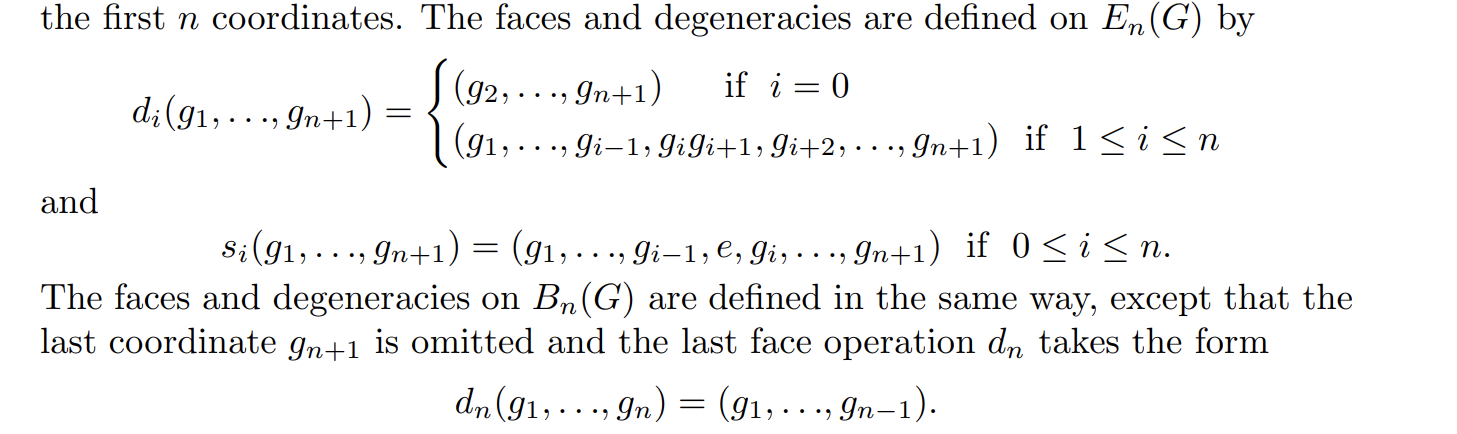
\includegraphics[scale=0.3]{face.png}
\end{figure}

此时$p_*$是自然的单纯集映射。

所谓分类空间,是指$E_*$和$B_*$的几何实现$E(G)$和$B(G)$。此时自然有空间之间的连续映射$p:E(G) \to B(G)\quad p(|(e_0,\dots,e_n),u|)=|e_0,\dots,e_{n-1},u|$。

我们仔细考察一下两个空间的结构。$E(G)$满足:
\begin{align*}
    E(G)^n -E(G)^{n-1}=(G^n-W)\times G \times (\Delta_n-\partial \Delta_n)\\
    B(G)^n -B(G)^{n-1}=(G^n-W)\times (\Delta_n-\partial \Delta_n)\\
\end{align*}
其中$W$是这样的$G^n$的子集:至少有一个坐标为$e$的点。自然,我们会有猜想:
\begin{proposition}
    $(p,E(G),B(G),G)$是一个纤维丛。
\end{proposition}
这个猜想正确的可能性很大——若$e$是$G$的非退化点,即$e \to G$是上纤维。这里我们不给出证明。而下一个命题则没有那么自然,尽管我们一样不能给出证明。
\begin{proposition}
    $E(G)$是可缩空间。
\end{proposition}

根据纤维丛诱导的长正合列:
\begin{align*}
    \dots \to 0=\pi_{q+1}(E(G)) \to \pi_{q+1}(B(G)) \to \pi_{q}(G) \to \pi_q(E(G))=0 \to \dots
\end{align*}
我们得到:
\begin{align*}
    \pi_{q+1}(B(G))\cong \pi_q(G)
\end{align*}

对于拓扑群$G$和$H$,下面的群同构,空间同胚显然:
\begin{align*}
    (G \times H)^n \cong G^n \times H^n
\end{align*}

于是单纯集合的同构显然:
\begin{align*}
    E_*(G \times H)\cong E_*(G) \times E_*(H),\quad B_*(G \times H)\cong B_*(G) \times B_*(H)
\end{align*}

由于几何实现是同胚,因此:
\begin{align*}
    B(G\times H)\cong B(G)\times B(H)
\end{align*}

现在假设$G$是交换的群,因此乘法$G \times G \to G$和取逆$G \times G$都是群同态。
\begin{proposition}
    $B(G)$和$E(G)$是交换的拓扑群。
\end{proposition}
\begin{proof}
    仅证明$B(G)$。我们直接考虑:
    \begin{align*}
        B(G)\times B(G) \cong B(G \times G) \to B(G)
    \end{align*}

    因为$G$交换,所有上述乘法交换。实际上我们需要讨论幺元和逆元。但是这涉及到几何实现的同胚。这是我们没有讨论的,因而暂且作罢。
\end{proof}

此外,$p:E(G) \to B(G)$也是同态。$G$对$E(G)$的嵌入(以$B_0(G)$唯一点作为原像集合生成的$G$)也是同态。

\begin{definition}
    设$B^0(G)=G$。$B^n(G)=B^{n-1}(G)$。对于abel群$\pi$,定义其拓扑为离散拓扑,则其零阶同伦群为$\pi$。我们定义Eilenberg-MacLane空间:
    \begin{align*}
        K(\pi,n)=B^n(\pi)
    \end{align*}
    不难根据$\pi_{q+1}(B(G)) \cong \pi_q(G)$逐步降低,最后得到$K$满足我们对Eilenberg-MacLane空间的期待。
\end{definition}
\section{Poincare对偶定理}
在把代数拓扑的结果运用到几何拓扑的研究中,Poincare对偶定理是一个关键的里程碑。其给出紧致流形的同调与上同调的关系。这完全是拓扑意义上的。
\subsection{前置知识}
在叙述Poincare对偶定理前,我们需要给出一些前置的知识。
\subsubsection{帽积(cap product)}
我们已经知道,上同调具有cup product。其本质是复合$H^q(X)$和$H^{p}(X)$而得到$H^{p+q}(X)$。这里的关键是对角映射$X \to X\times X$使得我们可以把$X \times X$的上同调映射到$X$中。

设$X$是CW复形。同样考虑$\Delta:X \to X \times X$。其并非是胞腔映射,于是我们考虑其CW逼近$\Delta'$.因此:
\begin{align*}
    \Delta'_*: C_*(X) \to C_*(X \times X) \cong C_*(X) \otimes C_*(X)
\end{align*}
具体的说,则$C_n(X)$的元素被映射到$\sum C_p(X) \otimes C_{n-p}(X)$中。

与$R$做张量积:
\begin{align*}
    \Delta'_*: C_*(X;R) \to C_*(X \times X;R) \cong C_*(X;R) \otimes C_*(X;R)
\end{align*}
对于一个$R$模,我们定义$\cap:C^*(X;\pi)\otimes C_*(X;R) \to C_*(X;\pi)$:
\begin{align*}
    C^*(X;\pi) \otimes_R C_*(X;R) \stackrel{\mathrm{id}\otimes \Delta_*'}{\longrightarrow}C^*(X;R)\otimes C_*(X;R) \otimes C_*(X;R) \stackrel{\epsilon \otimes \mathrm{id}}{\longrightarrow}C_*(X;\pi)
\end{align*}
具体的,我们把:
\begin{align*}
    Hom_R(C_p(X;R),\pi)\otimes_R C_p(X;R) \to \pi
\end{align*}
从而:
\begin{align*}
    \cap:C^p(X;\pi) \otimes_R C_n(X;R) \longrightarrow C_{n-p}(X;\pi)
\end{align*}
如果我们把上同调的链复形看作负的次数,则我们希望$\cap$是一个链复形之间的映射。实际上,只需要验证$\epsilon$是。然而$\epsilon \circ d=0$,所以即可。

因此$\cap$随即诱导了一个重要的映射:
\begin{align*}
    \cap: H^*(X;\pi) \otimes_R H_*(X;R) \rightarrow H_*(C^*(X;\pi)\otimes_R C_*(X;R)) \to H_*(X;\pi)
\end{align*}
这就是帽积的定义。

注意到帽积和杯积的最核心映射都是$\Delta:X \to X\times X$对角映射。所以我们自然猜想其有很强的关系。首先,杯积的定义为:
\begin{align*}
    \Delta'^*:C^*(X;R)\otimes C^*(X;R) \cong C^*(X \times X;R)\to C^*(X;R)
\end{align*}
我们考虑下面的交换图:\begin{tikzcd}
	{C^*(X\times X;R)\otimes_R C_*(X;R)} && {C^*(X\times X;R)\otimes_R C_*(X\times X;R)} \\
	\\
	{C^*(X;R)\otimes_RC_*(X;R)} && R
	\arrow["{id \otimes \Delta'_*}", from=1-1, to=1-3]
	\arrow["{\Delta'^*\otimes id}"', from=1-1, to=3-1]
	\arrow["\epsilon"', from=3-1, to=3-3]
	\arrow["\epsilon", from=1-3, to=3-3]
\end{tikzcd}

其中$\epsilon$是结合映射。交换的原因是我们把$C^*(X\times X;R)$写为$\mathrm{Hom}(C_*(X \times X),R)$。因此$\Delta'^*$和$\Delta'_*$有显而易见得关系。

我们断言杯积和帽积的关系是:
\begin{proposition}[基本恒等式]
    \begin{align*}
        \langle \alpha \cup \beta,x\rangle=\langle \beta,\alpha \cap x\rangle
    \end{align*}
\end{proposition}
\begin{proof}
    根据上述交换图。设$\langle \alpha \cup \beta,x\rangle$意指先走下,再走右。$\langle \beta,\alpha \cap x\rangle$意指先走右,再走下面。(有一个简单的交换关系,可参见教材。)
\end{proof}
在Poincare对偶定理的证明中,我们还需要用到相对帽积.对于$(X,A)$,我们有两种相对帽积:
\begin{align*}
     \cap: H^p(X,A;\pi) \otimes_R H_n(X,A;R) \to H_{n-p}(X;\pi)\quad \cap: H^p(X;\pi) \otimes_R H_n(X,A;R) \to H_{n-p}(X,A;\pi)
\end{align*}
假定$(X,A)$是CW复形对,$\Delta':A \to A \times A$同伦于对角映射。($M\otimes M /N \otimes N\cong M/N \otimes M$)
\begin{align*}
    \Delta'_*:C_*(X,A;R) \to C_*(X,A;R)\otimes C_*(X;R) \quad \Delta'_*:C_*(X,A;R) \to C_*(X;R)\otimes C_*(X,A;R)
\end{align*}

帽积的定义是明晰的,但是其困难在于难以用图的方式去追踪具体的点。
\subsubsection{定向和基本类}
在流形课程中我们学习了定向的定义。这里我们引入以某个交换环$R$为系数的定向。原来的定向可以看为$\R$系数的定向。我们先给出一个事实,然后介绍定向的定义。
\begin{proposition}
任何流形总是$\Z_2$可定向的。
\end{proposition}

对于$x \in M$,选取局部坐标邻域$U$,则根据正合公理和Excision公理:
\begin{align*}
    H_i(M,M-x)\cong H_i(U,U-x) \cong \tilde{H_{i-1}}(U-x) \cong \tilde{H}_{i-1}(S^{n-1})
\end{align*}
于是如果$i$不等于$n$,则$H_i(M,M-x)$是$0$.而$H_n(M,M-x)$是$R$。因此我们可以把$H_n(M,M-x)$看作一个生成元的$R$自由模。

\begin{definition}
    $M$的一个在子空间$X$处的$R$基本类意指$z_n \in H_n(M,M-X)$使得对于$\forall x \in X$,映射:
    \begin{align*}
        H_n(M,M-X)\to H_n(M,M-x)
    \end{align*}
    给出的$z_n$的像是$H_n(M,M_x)$的一个生成元。若$X=M$,则$z \in H_n(M)$简称为$M$的一个基本类。

    $M$的一个$R$-定向意指$M$的一个开覆盖$\{U_i\}$,使得每个$U_i$都有一个基本类$z_i$满足:$U_i \cap U_j$非空,则$z_i$和$z_j$被映射到$H_n(M,M-U_i\cap U_j)$的同一个元素。

    若$M$有一个$R$-定向,称其是可定向的。若$R=\Z$,则上述定义与流形的定向定义一致。
\end{definition}

关于定向的相关拓展,可查看\href{http://www.map.mpim-bonn.mpg.de/Orientation_of_manifolds}{网站}.

如果$M$本身有一个$R$-基本类,则其拥有一个自然的$R$-定向。我们只需要把开覆盖$\{U_i\}$中的$z_i$设置为$z$在映射$H_n(M) \to H_n(M,M-U_i)$下的像即可。根据$H_n$函子性,则自然给出定向。然而反过来则不那么容易。在紧致流形的情况下,这是正确的。为了说明此事,我们先给出定理:
\begin{theorem}[Vanishing]
    $M$是流形。对于系数群$\pi$,若$i>n$,则$H_i(M;\pi)=0$。若$M$连通但不紧致,则$\tilde{H}_n(M;\pi)=0$。
\end{theorem}
证明在下节给出。根据消失定理和MV序列,我们给出:

\begin{theorem}
    设$K$是$M$的紧子空间。则对于任何系数群$\pi$,$H_i(M,M-K;\pi)=0$,若$i>n$。并且一个$M$的$R$-定向唯一决定$M$在$K$上的一个基本类。特别的,若$M$是紧的,则$R$-定向决定一个基本类。
\end{theorem}
\begin{proof}
    首先假定$K$被包含在一个局部坐标邻域$U$中。于是:
    \begin{align*}
        H_i(M,M-K;\pi)\cong H_i(U,U-K;\pi) \cong \tilde{H}_{i-1}(U-K;\pi)
    \end{align*}
    由于$U-K$是开集,所以根据消失定理,在$i>n$的时候,$\tilde{H}_{i-1}(U-K;\pi)=0$.想要给出$K$处的基本类,则考虑$M$在$U$处的基本类。$H_n(M,M-U) \to H_n(M,M-K)$给出$K$处的基本类。

    为了给出一般的结果,我们只需要说明,若结论已经对$K,L,K\cap L$成立,则对$K\cup L$也成立。为此,考虑MV序列:
    \begin{align*}
        H_{i+1}(M,M-K\cap L) \to H_i(M,M-K\cup L) \stackrel{\psi}{\rightarrow} H_i(M,M-K)\oplus H_i(M,M-L) \stackrel{\phi}{\rightarrow} H_i(M,M-K\cap L)
    \end{align*}
    若$i>n$,则长正合列给出$H_i(M,M-K\cup L)=0$。设$i=n$,则根据$H_{i+1}=0$得知$\psi$是单射。显然同一个定向给出的$K$和$L$的基本类$z_K$和$z_L$是相容的,则$\phi(z_K,z_L)=0$.根据正合性存在唯一的$z_{K\cup L}$使得$\psi(z_{K\cup L})=(z_K,z_L)$。

    显然$z_{K \cup L}$是$K\cup L$的基本类。
\end{proof}

在定向方面,我们还有一个有意思的结论:
\begin{corollary}
    设$M$是连通的紧致流形,维度大于$0$.则要么$M$是不可定向的,并且$H_n(M;\Z)=0$。要么$M$可定向且:
    \begin{align*}
        H_n(M;\Z) \rightarrow H_n(M,M-x;\Z)\cong \Z
    \end{align*}
\end{corollary}
\begin{proof}
    观察$H_n(M-x)$.这是一个连通但不紧致的流形,所以消失定理告诉我们这是0调。因此根据正合公理:
    \begin{align*}
        H_n(M;\pi) \rightarrow H_n(M,M-x;\pi)\cong \pi
    \end{align*}
    是一个典范的单射。由于$\Z_q$是域,根据泛系数定理,我们有单射:
    \begin{align*}
        H_n(M;\Z)\otimes Z_q \to H_n(M,M-x;\Z)\otimes Z_q \cong Z_q,
    \end{align*}
    对于任何$q$都成立。若$H_n(M;\Z)$不是$0$,则上述单射是同构。定向的关系是一目了然的。
\end{proof}
\subsubsection{消失定理的证明}
本节我们简单证明消失定理。当然详细的证明请参见教材。

\begin{lemma}[同调的紧支性]
    对于任何空间$X$和元素$x \in H_q(X)$,存在$X$的紧子空间$K$和$k \in H_q(K)$使得$k$被映射到$x$。
\end{lemma}
\begin{proof}
    考虑$Y$是$X$的CW逼近。记$x=\gamma_*(y)$。考虑$y$在$C_q(X)$中的代表元$z$。则$z$是有限多个$q$胞腔的和,是$C_q(L)$($L$是$Y$的一个有限子复形)中的元素。设$K=\gamma(L)$并且$k$是$z$的同调类在$\gamma$下的像,则$K$是紧空间,并且$k$的像是$x$。(CW逼近是一个函子)
\end{proof}
\begin{lemma}
    设$U$是$\R^n$的开集,则$H_i(U)=0$,若$i \geq n$。
\end{lemma}
\begin{proof}
    设$s \in H_i(U)$。我们说明$i \geq n$的时候$s=0$。根据上面的引理,存在紧集$K$满足$k \in H_i(K)$且$i_*:H_i(K)\to H_i(U)$有$i_*(k)=s$。

    考虑$\R^n$的一个精细的CW结构:由小的n-立方体构成n胞腔,则$K$是紧集意蕴存在一个有限的子复形$L:K \subset L \subset U$。考虑交换图:
    \begin{tikzcd}
	{H_{i+1}(\R^n,L)} & {H_i(\R^n,U)} \\
	{H_i(L)} & {H_i(U)}
	\arrow[from=1-1, to=2-1]
	\arrow[from=2-1, to=2-2]
	\arrow[from=1-1, to=1-2]
	\arrow[from=1-2, to=2-2]
\end{tikzcd}

    注意到当$i \geq n-1$的时候$(\R^n,L)$的同调显然是$0$。从而交换图左边为$0$。而$s$在$H_i(L)$的像中(先映射到$H_i(L)$,再到$H_i(U)$)。从而$s=0$。
\end{proof}
\begin{lemma}
    设$U$是$\R^n$中的开集。假定$t \in H_n(\R^n,U)$,且任意$x \in \R^n-U$,都有$t$被映射到$H_n(\R^n,\R^n-x)$中的$0$。则$t=0$。
\end{lemma}
\begin{proof}
    定理的约化版本:若$s \in \tilde{H}_{n-1}(U)$且对于任意$x \in \R^n-x$,都有$s$被映射到$\tilde{H}_{n-1}(\R^n-x)$中的$0$,则$s=0$。

    同样考虑$K$紧集。则$K$包含在一个略大的开集$\tilde{V}$中,且$\overline{V}$是紧集,$\overline{V} \subset K$.于是我们有一个开集$V$使得$s$在$r \in \tilde{H}_{n-1}(V)$的像中。我们断言$r$的像是$0$.

    我们考虑$V$被一个可缩空间$T$包含,且$T$的闭包仍是紧集。记$L=T-(T\cap U)$。对于$x \in \overline{L}$,考虑一个闭的方体$D$包裹$x$。则有限覆盖告诉我们,存在$\{D_1,\dots,D_q\}$满足覆盖$\overline{L}$。

    设$C_i=D_i \cap T$.我们断言,$r$在$\tilde{H}_{n-1}(T-(C_1\cup \dots \cup C_p))$,$0 \leq p \leq q$的像是$0$。这通过归纳得到。

    若$p=0$,则$\tilde{H}_{n-1}(T)$是$0$。于是显然。对于归纳步骤,我们给出MV序列:
    \begin{align*}
        \tilde{H}_{n-1}(T-(C_1\dots C_p)) \to \tilde{H}_{n-1}(T-(C_1\dots C_{p-1}))\oplus \tilde{H}_{n-1}(\R^n-D_p)
    \end{align*}
    是一个单射。因为$\tilde{H}_n(T-(C_1\cup \dots C_{p-1}))\cup (\R^n-D_p)$是$0$。(开集的同调在$i \geq n$时为$0$。)

    注意到$s$映射到右边两个同调群都是$0$(归纳假设和$D_p$可以缩到$U$外的点)。所以归纳步骤完成。
    \begin{align*}
        V \subset T-(C_1\cup \dots \cup C_q)\subset T\cap U \subset U
    \end{align*}
    告诉我们$r$的像是$0$。
\end{proof}
用上面三个引理,我们给出消失定理的sketch of proof.
\begin{proof}[sketch of proof of vanishing theorem]
    设$s \in H_i(M)$。我们必须说明若$i >n$,$s=0$.若$M$连通但不紧且$i=n$,$s=0$.

    考虑$M$的紧子空间使得$s$属于$H_i(K)$的像中。则$K$被有限个局部坐标邻域$\{U_i\}$覆盖。根据函子性,要说明$s=0$,只需要说明$H_i(U_1\cup \dots \cup U_q)=0$。

    我们自然可以做数学归纳。因此我们要说明对于特定的$i$值,$H_i(U \cup V)=0$。条件是$U$是局部坐标,而$V$是在$i$特定值情况下$H_i(V)=0$的开集。自然是考虑MV序列:
    \begin{align*}
        H_i(U) \oplus H_i(V) \to H_i(U \cup V) \to \tilde{H}_{i-1}(U\cap V) \to \tilde{H}_{i-1}(U)\oplus \tilde{H}_{i-1}(V)
    \end{align*}
    首先考虑$i>n$的情况。此时,$U\cap V$是$\R^n$开集,所以$H_i(U\cup V)$两边总是$0$。因此$H_i(U\cup V)=0$。

    现在假设$M$是连通的不紧开集,并且赋值$i=n$。我们首先有$H_n(U)=0$,$H_n(V)=0$,$\tilde{H}_{n-1}(U)=0$.根据MV序列,$H_n(U\cup V)=0$等价于$\tilde{H}_{n-1}(U\cap V) \to \tilde{H}_{n-1}(V)$是单射。这个映射由映入映射$U\cap V \to V$诱导。

    我们断言,$H_n(M) \to H_n(M,M-y)$对于$\forall y \in M$都是零同态。若$x \in M$并且$L$是一条连接$x$和$y$的道路,则交换图:
    \begin{tikzcd}
	&& {H_n(M,M-x)} \\
	{H_n(M)} & {H_n(M,M-L)} \\
	&& {H_n(M,M-y)}
	\arrow["\cong", from=2-2, to=1-3]
	\arrow["\cong", from=2-2, to=3-3]
	\arrow[from=2-1, to=2-2]
    \end{tikzcd}成立。
    
    上述交换图表明,如果$s \in H_n(M)$被映射到$H_n(M,M-x)$中的$0$,则也映射到$H_n(M,M-y)$中的$0$.因此我们只需要说明有一个$x$即可。如果$s$处于$H_n(K)$的像中,$K$是紧集,我们可以选择$x \in M-k$使得$K \to M \to (M,M-x)$正合。因此$s$被映射到$H_n(M,M-x)$中的$0$.

    考虑下面的交换图。
    \begin{figure}[htbp]
        \centering
        \begin{tikzcd}
	&& {H_n(U\cup V)} & {H_n(M)} \\
	{H_n(V,U\cap V)} & {H_n(U\cup V,U\cap V)} && {H_n(M,M-y)} \\
	{\tilde{H}_{n-1}(U\cap V)} & {H_n(U,U\cap V)} && {H_n(U,U-y)} \\
	{\tilde{H}_{n-1}(V)}
	\arrow[from=1-3, to=1-4]
	\arrow["0", from=1-4, to=2-4]
	\arrow["\cong"', from=3-4, to=2-4]
	\arrow[from=3-2, to=3-4]
	\arrow["\partial"{description}, from=3-2, to=3-1]
	\arrow["{i_*}", from=3-1, to=4-1]
	\arrow["\partial"{description}, from=2-1, to=3-1]
	\arrow[from=2-1, to=2-2]
	\arrow[from=1-3, to=2-2]
	\arrow["\partial"{description}, from=2-2, to=3-1]
	\arrow[from=3-2, to=2-2]
	\arrow[from=2-2, to=2-4]
    \end{tikzcd}
    \end{figure}
    我们的目的是说明图中$i_*$是单射。设$r \in \ker i_*$。注意到$\tilde{H}_{n-1}(U)=0$,则最下方的$\partial$是满射。所以存在$s \in H_n(U,U\cap V)$使得$\partial(s)=r$。我们的目的是说明$s=0$。

    观察$s$,其位于$H_n(U,U\cap V)$。我们只需要说明对于任何$y \in U-(U\cap V)$,都有$s$映射到$H_n(U,U-y)$中的$0$.根据引理可以得到$s=0$。

    在$H_n(V,U\cap V)$中存在$t$使得$\partial(t)=r$。用$t'$和$s'$代表原字母在$H_n(U\cup V,U\cap V)$中的像。于是$\partial(t'-s')=0$,意蕴着$w \in H_n(U\cup V)$。

    从$w$出发,映射到$H_n(M,M-y)$为$0$意味着$s'-t'$也是。

    注意到$t$映射到$H_n(M,M-y)$是$0$,所以$s$也是。因此$s$映射到$H_n(U,U-y)$也是$0$。从而命题得证。
\end{proof}
\subsection{Poincare对偶定理}
\begin{theorem}[Poincare对偶定理]
    设$M$是紧致$R$-定向流形。则对于任何的$R$模$\pi$,下面的映射$D$是一个同构:
    \begin{align*}
        D:H^p(M;\pi)\cong H_{n-p}(M;\pi)
    \end{align*}
    其中,$D$由$D(\alpha)=\alpha \cap z$给出,$z$是$M$的基本类。
\end{theorem}
回忆基本恒等式(仅仅在系数为$R$的情况下成立):
$$
\langle \alpha \cup \beta,x\rangle=\langle \beta,\alpha \cap x\rangle
$$
因此$D$甚至是杯积的伴随。

现在我们证明定理。
\begin{proof}
    略
\end{proof}
\subsection{一些应用}
\subsubsection{方向覆盖}
这小节我们采取整系数的同调。
\begin{proposition}
    设$M$是连通$n$流形。则存在一个2覆叠$p:\tilde{M}\to M$使得$\tilde{M}$是连通的当且仅当$M$不是可定向的。
\end{proposition}
\begin{proof}
    仅仅记录构造方法:
    \begin{align*}
        \tilde{M}=\{(x,\alpha)|x \in M,\alpha(\text{生成元}) \in H_n(M,M-x)\}, \quad p(x,\alpha)=x
    \end{align*}
    $\tilde{M}$的拓扑基为:$U$为开集,$\beta \in H_n(M,M-U)$
    $$
    \langle U,\beta\rangle=\{(x,\alpha)|x \in U,\beta \text{被映射为}\alpha\}
    $$
    事实上,若$(x,\alpha)\in \langle U,\beta\rangle \cap \langle V,\gamma \rangle$,则可以选择坐标邻域$W:x \in W$。并且存在唯一的$\alpha'$使得$\alpha' \in H_n(M,M-W)$映射到$\alpha$,且$\alpha,\beta$映射到$\alpha'$。

    显然$\tilde{M}$是流形且是2覆叠。我们接下来说明$\tilde{M}$可定向。实际上,如果$U$是一个局部坐标,$(x,\alpha)\in \langle U,\beta \rangle$,下面的映射图诱导了同构:
    \begin{figure}
        \centering
        \begin{tikzcd}
	    {(\tilde{M},\tilde{M}-\langle U,\beta\rangle)} & {(M,M-U)} \\
	    {(\tilde{M},\tilde{M}-(x,a))} & {(M,M-x)} \\
	    {(\langle U,\beta\rangle,\langle U,\beta\rangle-(x,\alpha))} & {(U,U-x)}
	    \arrow[from=1-1, to=2-1]
	    \arrow[from=3-1, to=2-1]
	    \arrow["{p }", from=3-1, to=3-2]
	\arrow[from=3-2, to=2-2]
	\arrow[from=1-2, to=2-2]
    \end{tikzcd}
    \end{figure}
    通过这个图,$\beta \in H_n(M,M-U)$具体了一个$\tilde{\beta}\in H_n(\tilde{M},\tilde{M}-\langle U,\beta\rangle)$,并且独立于$(x,\alpha)$的选择。

    对于开集$U$,只需要指定其定向为$\beta$即可。

    根据定义,$M$的一个定向是一个特殊的截面$s:M \to \tilde{M}$。改变符号,$-s$表明$\tilde{M}=\mathrm{im}(s)\cup \mathrm{im}(-s)$且不交。如果$M$可定向,则$\tilde{M}$写为两个同胚于$M$的不交并。$\tilde{M}$不连通。
    
    如果$M$不可定向,则$\tilde{M}$连通。假设$\tilde{M}$不连通,则存在$(x,\alpha)$和$(x,-\alpha)$在两个连通分支。容易说明这两个连通分支给出了定向。
\end{proof}
\begin{proposition}
    如果$M$是单连通的,或者$\pi_1(M)$不包含指数为$2$的子群,则$M$是可定向的。如果$M$可定向,则$M$有且仅有两个方向。
\end{proposition}
\begin{proof}
    如果$M$不可定向,则$p_*(\pi_1(\tilde{M}))$是$\pi_1(M)$的指数为$2$的子群。着给出了第一个命题。第二个命题实属显然。
\end{proof}
\subsubsection{一些推论}
考虑整数系数,则根据对偶,$H^p(M)\cong H_{n-p}(M)$。若$p=0$,则$H^0(M)\cong H_n(M)$。于是$H_n(M)=\Z$.注意到同构由:
\begin{align*}
    D:H^0(M) \to H_n(M): D(\alpha)=\alpha \cap z
\end{align*}
给出。此时$H_n(M)$的生成元就是其基本类。因为基本类必须映射到$\Z$的$1$。

若$p=n$,则$H_0(M)\cong H^n(M)=\Z$。我们也得到了$H^n(M)$的生成元$\zeta$。并且$\zeta$和$z$对偶:$\langle \zeta,z\rangle=1$。(用奇异同调清楚知道$H_0$和$H^0$的情况。)

\begin{corollary}
    设$T_p$是$H^p(M)$的挠子群。杯积$\alpha \otimes \beta$给出$\langle \alpha\beta,z\rangle$给出了非奇异的双线性:
    \begin{align*}
        H^p(M)/T_p \otimes H^{n-p}(M)/T_{n-p}\to \Z
    \end{align*}
\end{corollary}
\begin{proof}
    若$\alpha \in T_p$,则存在$ra=0$。从而$r(\alpha \cup \beta)=0$。因为$H^n(M)\cong \Z$,则$\alpha \cup \beta=0$。因此杯积在挠元的时候为$0$。上述映射是良定的。

    注意到$\mathrm{Ext}_{\Z}^1(\Z_r,\Z)=\Z_r$,并且$H_p(M)$一定是有限生成的,则$\mathrm{Ext}_{\Z}^1(H_*(M),\Z)$是一个挠群。从而根据泛系数定理,由:
    \begin{align*}
        H^p(M)/T_p\cong \mathrm{Hom}(H_p(M),\Z)
    \end{align*}
    若$\alpha \in H^p(M)$投射到自由abel群$H^p(M)/T_p$的一个生成元,则存在$\alpha \in H_p(M)$使得$\langle \alpha,a\rangle=1$。用对偶,则存在$\beta \in H^{n-p}(M)$使得$\beta \cap z=a$:$\langle \beta \cup \alpha,z\rangle=\langle \alpha,\beta \cap z\rangle=1$
\end{proof}

借此,我们甚至可以给出$\C P^n$的杯积。(给出上同调环)
\begin{corollary}
    作为分次环,$H^*(\C P^n)$是多项式代数$Z[\alpha]/)\alpha^{n+1}$,其中$\alpha$的度是$2$.
\end{corollary}
\begin{proof}
显然$H^{2q}(\C P^n)$是自由Abelian群,其生成元只有一个。$0\leq q \leq n$。我们要说明的是$H^{2q}(\C P^n)$的生成元是$\alpha^q$.

注意到$\C P^{n-1}$是$\C P^{n}$的$2n-1$骨架,所以显然有同构:$H^{2q}(\C P^n) \to H^{2q}(\C P^{n-1})$在$q<n$时候的同构。根据$n$进行归纳。当$n=1$,$\C P^1 \cong S^2$。此时结论是平凡的。

现在假定$n-1$成立。从而$q<n$时,$\alpha^q$生成了$H^{2q}(\C P^n)$。根据上面的推论,注意到存在$H^{2q-2}(\C P^n)$使得$\alpha \cup \beta$与$z$做内积为$1$。而$\alpha \cup \beta$显然是$H^{2n}(M)$的生成元,因此我们只需要说明$\beta$是$H^{2q-2}$的生成元。实际上这是明显的,因为$\beta$来自于$H_2(M)$的生成元。
\end{proof}
考虑到$M$的上同调中的挠元,更方便的是考虑$R$是一个域。
\begin{proposition}
    任何可定向流形$M$对于交换环$R$来说都是$R$可定向的。
\end{proposition}
\begin{proposition}
    设$M$是连通的紧致$R$定向流形,其中$R$是域。则$\alpha \otimes \beta \to \langle \alpha\cup \beta,z\rangle$定义了非奇异的映射:
    \begin{align*}
        H^p(M;R)\otimes_R H^{n-p}(M;R)\to R
    \end{align*}
\end{proposition}
最后的推论是:
\begin{corollary}
    作为分次环,$H^*(\R P^n;\Z_2)$是多项式$Z_2[\alpha]/(\alpha^{n+1})$。其中$\alpha=1$,即$\alpha^q$是$H^q(\R P^n;\Z_2)$的非零元。
\end{corollary}
\end{document}



